% !Mode:: "TeX:UTF-8"

\def\usewhat{xelatex} % 定义编译方式 pdflatex, dvipdfmx, or xelatex

\def \xuewei{Doctor} % 定义学位 Doctor or Master

\def\xueke{Engineering} % 定义学科 Engineering, Science, Management, Arts, Philosophy, Economics, Laws, Education, or History

\documentclass[cs4size,openany,twoside,UTF8,normalindentfirst,nofonts]{ctexbook}

% !Mode:: "TeX:UTF-8" 

\makeatletter
\@tempcnta=128
\loop \catcode\@tempcnta=13 \ifnum\@tempcnta<255 \advance \@tempcnta \@ne
\repeat
\makeatother

\newif\ifxueweidoctor %判断论文类型
\newif\ifxueweimaster
\def\temp{Doctor}
\ifx\temp\xuewei
  \xueweidoctortrue  \xueweimasterfalse
\fi
\def\temp{Master}
\ifx\temp\xuewei
  \xueweidoctorfalse  \xueweimastertrue
\fi

\ifxueweidoctor
  \newcommand{\cxuewei}{博士}
  \newcommand{\exuewei}{Doctor}
  \newcommand{\exueweier}{Doctoral}
  \newcommand{\xueweishort}{博}
\fi

\ifxueweimaster
  \newcommand{\cxuewei}{硕士}
  \newcommand{\exuewei}{Master}
  \newcommand{\exueweier}{Master's}
  \newcommand{\xueweishort}{硕}
\fi    % 硕博类型

% !Mode:: "TeX:UTF-8" 
\usepackage{xeCJK}
\usepackage{tabularx}
\usepackage{graphicx}
%\usepackage[a4paper,text={150true mm,224true mm},top=35.5true mm,left=30true mm,head=5true mm,headsep=2.5true mm,foot=8.5true mm]{geometry}       %哈工大原版



\usepackage[a4paper,top=35true mm,bottom=30true mm,left=31.7true mm,right=31.7true mm,headsep=3true mm,foot=8true mm]{geometry}       %哈医大2014版
\xeCJKsetup{AutoFakeBold=4}%伪粗程度控制
\setlength{\baselineskip}{24pt}%基本行距默认12pt,此为双倍行距


\usepackage{titlesec}               % 控制标题的宏包
\usepackage{array}		%表格固定列宽 居中
\usepackage{titletoc}                   % 控制目录的宏包
\usepackage{fancyhdr}                   % fancyhdr宏包 页眉和页脚的相关定义aTeX宏包 用来排aTeX宏包 用来排
\usepackage{color}          % 支持彩色
\usepackage{amsmath}        % AMSLaTeX宏包 用来排出更加漂亮的公式
\usepackage{amssymb}
\usepackage[below]{placeins}%允许上一个section的浮动图形出现在下一个section的开始部分,还提供\FloatBarrier命令,使所有未处理的浮动图形立即被处理
\usepackage{flafter}       % 使得所有浮动体不能被放置在其浮动环境之前,以免浮动体在引述它的文本之前出现.
\usepackage{multirow}       %使用Multirow宏包,使得表格可以合并多个row格
\usepackage{booktabs}       % 表格,横的粗线;\specialrule{1pt}{0pt}{0pt}
\usepackage{longtable}      %支持跨页的表格。
\usepackage[hang]{subfigure}%支持子图 %centerlast 设置最后一行是否居中
\usepackage[subfigure]{ccaption} %支持双语标题
\usepackage[sort&compress,numbers]{natbib}% 支持引用缩写的宏包
\usepackage{enumitem}       %使用enumitem宏包,改变列表项的格式
\usepackage{calc}           %长度可以用+ - * / 进行计算
%\usepackage{txfonts}
\usepackage{fontspec}
\usepackage[amsmath,thmmarks,hyperref]{ntheorem}% 定理类环境宏包,其中 amsmath 选项用来兼容 AMS LaTeX 的宏包
\usepackage{etoolbox}
\AtBeginDocument{%
  \apptocmd\thebibliography{\interlinepenalty=-5000 }{}{}%
}

% 生成有书签的pdf及其开关, 该宏包应放在所有宏包的最后, 宏包之间有冲突
\def\atemp{dvipdfmx}\ifx\atemp\usewhat
\usepackage[dvipdfmx,unicode,           %dvi-->pdf 生成书签
            bookmarksnumbered=true,
            bookmarksopen=true,
            colorlinks=false,
            pdfborder={0 0 1},
            citecolor=blue,
            linkcolor=red,
            anchorcolor=green,
            urlcolor=blue,
            breaklinks=true
            ]{hyperref}
\fi

\def\atempxetex{xelatex}\ifx\atempxetex\usewhat %\def\atempxetex{xelatex} main.tex中已定义;
\usepackage[xetex,
            bookmarksnumbered=true,
            bookmarksopen=true,
            colorlinks=false,
            pdfborder={0 0 1},
            citecolor=blue,
            linkcolor=red,
            anchorcolor=green,
            urlcolor=blue,
            breaklinks=true,
            naturalnames  %与algorithm2e宏包协调
            ]{hyperref}

\defaultfontfeatures{Mapping=tex-text}
\xeCJKsetemboldenfactor{1}%只对随后定义的CJK字体有效
\setCJKfamilyfont{hei}{SimHei}
\xeCJKsetemboldenfactor{4}
\setCJKfamilyfont{song}{SimSun}
\xeCJKsetemboldenfactor{1}
\setCJKfamilyfont{fs}{FangSong}
\setCJKfamilyfont{kai}{KaiTi}
\setCJKfamilyfont{li}{LiSu}
\setCJKfamilyfont{xw}{STXinwei}
\setCJKmainfont{SimSun}
\setCJKsansfont{SimHei}
\setmainfont{Times New Roman}
\setsansfont{Arial}
%哈医大要求黑/宋/楷(不知是否GB2312)/Times New Roman
\newcommand{\hei}{\CJKfamily{hei}}% 黑体   (Windows自带simhei.ttf)
\newcommand{\song}{\CJKfamily{song}}    % 宋体   (Windows自带simsun.ttf)
\newcommand{\fs}{\CJKfamily{fs}}        % 仿宋体 (Windows自带simfs.ttf)
\newcommand{\kaishu}{\CJKfamily{kai}}      % 楷体   (Windows自带simkai.ttf)
\newcommand{\li}{\CJKfamily{li}}        % 隶书   (Windows自带simli.ttf)
\newcommand{\xw}{\CJKfamily{xw}}        % 隶书   (Windows自带simli.ttf)
\newfontfamily\arial{Arial}
\newfontfamily\timesnewroman{Times New Roman}
\fi

\usepackage[boxed,linesnumbered,algochapter]{algorithm2e}  % 算法的宏包,注意宏包兼容性,先后顺序为float、hyperref、algorithm(2e),否则无法生成算法列表 
\usepackage{xltxtra}
\usepackage{listings}
\lstset{
%basicstyle=\small\ttfamily,
columns=flexible,
breaklines=true
}
\newcommand{\emultiline}[2][c]{\renewcommand{\arraystretch}{1}\begin{tabular}[#1]{@{}l@{}}#2\end{tabular} \renewcommand{\arraystretch}{1.3} }
\newcommand{\citeayu}[1]{\citeauthor{#1}~(\citeyear{#1})\citeup{#1}}
 % 引用的宏包

\graphicspath{{figures/}} %定义所有的eps文件在 figures 子目录下

\begin{document}

% !Mode:: "TeX:UTF-8" 

%\newcommand{\song}{\CJKfamily{song}}    % 宋体   (Windows自带simsun.ttf)
%\newcommand{\hei}{\CJKfamily{hei}}      % 黑体   (Windows自带simhei.ttf)
%\newcommand{\kaishu}{\CJKfamily{kai}}      % 黑体   (Windows自带simhei.ttf)

\newcommand{\yihao}{\fontsize{26pt}{26pt}\selectfont}       % 一号, 1.倍行距
\newcommand{\xiaoyi}{\fontsize{24pt}{24pt}\selectfont}      % 小一, 1.倍行距
\newcommand{\erhao}{\fontsize{22pt}{1.25\baselineskip}\selectfont}       % 二号, 1.倍行距
\newcommand{\xiaoer}{\fontsize{18pt}{18pt}\selectfont}      % 小二, 单倍行距
\newcommand{\sanhao}{\fontsize{16pt}{16pt}\selectfont}      % 三号, 1.倍行距
\newcommand{\xiaosan}{\fontsize{15pt}{15pt}\selectfont}     % 小三, 1.倍行距
\newcommand{\sihao}{\fontsize{14pt}{14pt}\selectfont}       % 四号, 1.0倍行距
\newcommand{\xiaosi}{\fontsize{12pt}{12pt}\selectfont}      % 小四, 1.倍行距
\newcommand{\wuhao}{\fontsize{10.5pt}{10.5pt}\selectfont}   % 五号, 单倍行距
\newcommand{\xiaowu}{\fontsize{9pt}{9pt}\selectfont}        % 小五, 单倍行距


%避免宏包 hyperref 和 arydshln 不兼容带来的目录链接失效的问题。
\def\temp{\relax}
\let\temp\addcontentsline
\gdef\addcontentsline{\phantomsection\temp}

\makeatletter
\gdef\hitempty{}

%重新定义BiChapter命令,可实现标题手动换行,但不影响目录
\def\BiChapter{\relax\@ifnextchar [{\@BiChapter}{\@@BiChapter}}
\def\@BiChapter[#1]#2#3{\chapter[#1]{#2}
    \addcontentsline{toe}{chapter}{\bfseries \xiaosi Chapter \thechapter\hspace{0.5em} #3}}
\def\@@BiChapter#1#2{\chapter{#1}
    \addcontentsline{toe}{chapter}{\bfseries \xiaosi Chapter \thechapter\hspace{0.5em}{\boldmath #2}}}

\newcommand{\BiSection}[2]
{   \section{#1}
    \addcontentsline{toe}{section}{\protect\numberline{\csname thesection\endcsname}#2}
}

\newcommand{\BiSubsection}[2]
{    \subsection{#1}
    \addcontentsline{toe}{subsection}{\protect\numberline{\csname thesubsection\endcsname}#2}
}

\newcommand{\BiSubsubsection}[2]
{    \subsubsection{#1}
    \addcontentsline{toe}{subsubsection}{\protect\numberline{\csname thesubsubsection\endcsname}#2}
}

\newcommand{\BiAppendixChapter}[2] % 该附录命令适用于发表文章,简历等
{\phantomsection
\markboth{#1}{#1}
\addcontentsline{toc}{chapter}{\xiaosi #1}
\addcontentsline{toe}{chapter}{\bfseries \xiaosi #2}  \chapter*{#1}
}

\newcommand{\BiAppChapter}[2]    % 该附录命令适用于有章节的完整附录
{\phantomsection 
 \chapter{#1}
 \addcontentsline{toe}{chapter}{\bfseries \xiaosi Appendix \thechapter~~#2}
}

\renewcommand{\thefigure}{\arabic{chapter}-\arabic{figure}}%使图编号为 7-1 的格式 %\protect{~}
\renewcommand{\thesubfigure}{\alph{subfigure})}%使子图编号为 a)的格式
\renewcommand{\p@subfigure}{\thefigure~} %使子图引用为 7-1 a) 的格式,母图编号和子图编号之间用~加一个空格
\renewcommand{\thetable}{\arabic{chapter}-\arabic{table}}%使表编号为 7-1 的格式
\renewcommand{\theequation}{\arabic{chapter}-\arabic{equation}}%使公式编号为 7-1 的格式

\newcommand{\algoenname}{Algo.} %算法英文标题
\newfloatlist[chapter]{algoen}{aen}{\listalgoenname}{\algoenname}
\newfixedcaption{\algoencaption}{algoen}
\renewcommand{\thealgoen}{\thechapter-\arabic{algocf}}
\renewcommand{\@cftmakeaentitle}{\chapter*{\listalgoenname\@mkboth{\bfseries\listalgoenname}{\bfseries\listalgoenname}}}

\renewcommand{\algorithmcfname}{算法}
\setlength\AlCapSkip{1.2ex}
\SetAlgoSkip{1pt}
\renewcommand{\algocf@captiontext}[2]{\wuhao#1\algocf@typo ~ \AlCapFnt{}#2} % text of caption
\expandafter\ifx\csname algocf@within\endcsname\relax% if \algocf@within doesn't exist
\renewcommand\thealgocf{\@arabic\c@algocf} % and the way it is printed
\else%                                    else
\renewcommand\thealgocf{\csname the\algocf@within\endcsname-\@arabic\c@algocf}
\fi
\renewcommand{\algocf@makecaption}[2]{%中英文双标题一定多于一行,因此去掉单行时的判断,并将\parbox中标题设置为居中
  \addtolength{\hsize}{\algomargin}%
  \sbox\@tempboxa{\algocf@captiontext{#1}{#2}}%
    \hskip .5\algomargin%
    \parbox[t]{\hsize}{\centering\algocf@captiontext{#1}{#2}}% 
  \addtolength{\hsize}{-\algomargin}%
}
\newcommand{\AlgoBiCaption}[2]{%直接取出自定义的中英文标题条目加入到真正的\caption 中  
   \caption[#1]{\protect\setlength{\baselineskip}{1.5em}#1 \protect \\ Algo. \thealgocf~~ #2} % \algoencaption{#2}   
   \addcontentsline{aen}{algoen}{\protect\numberline{\thealgoen}{#2}}
   }

\makeatother

%定义 学科 学位
\def \xuekeEngineering {Engineering}
\def \xuekeScience {Science}
\def \xuekeManagement {Management}
\def \xuekeArts {Arts}
\def \xuekePhilosophy {Philosophy}
\def \xuekeEconomics {Economics}
\def \xuekeLaws {Laws}
\def \xuekeEducation {Education}
\def \xuekeHistory {History}


\ifx \xueke \xuekeEngineering
\newcommand{\cxueke}{医学}
\newcommand{\exueke}{Engineering}
\fi

\ifx \xueke \xuekeScience
\newcommand{\cxueke}{理学}
\newcommand{\exueke}{Science}
\fi

\ifx \xueke \xuekeManagement
\newcommand{\cxueke}{管理学}
\newcommand{\exueke}{Management}
\fi

\ifx \xueke \xuekeArts
\newcommand{\cxueke}{文学}
\newcommand{\exueke}{Arts}
\fi 

\ifx \xueke \xuekePhilosophy
\newcommand{\cxueke}{哲学}
\newcommand{\exueke}{Philosophy}
\fi 

\ifx \xueke \xuekeEconomics
\newcommand{\cxueke}{经济学}
\newcommand{\exueke}{Economics}
\fi 

\ifx \xueke \xuekeLaws
\newcommand{\cxueke}{法学}
\newcommand{\exueke}{Laws}
\fi 

\ifx \xueke \xuekeEducation
\newcommand{\cxueke}{教育学}
\newcommand{\exueke}{Education}
\fi 

\ifx \xueke \xuekeHistory
\newcommand{\cxueke}{历史学}
\newcommand{\exueke}{History}
\fi 
 % 文本格式定义
% !Mode:: "TeX:UTF-8" 

\theoremstyle{plain}
\theorembodyfont{\song\rmfamily}
\theoremheaderfont{\hei\rmfamily}
\newtheorem{definition}{\hei 定义}[chapter]
\newtheorem{example}{\hei 例}[chapter]
\newtheorem{algo}{\hei 算法}[chapter]
\newtheorem{theorem}{\hei 定理}[chapter]
\newtheorem{axiom}{\hei 公理}[chapter]
\newtheorem{proposition}{\hei 命题}[chapter]
\newtheorem{lemma}{\hei 引理}[chapter]
\newtheorem{corollary}{\hei 推论}[chapter]
\newtheorem{remark}{\hei 注解}[chapter]
\newenvironment{proof}{\noindent{\hei 证明:}}{\hfill $ \square $ \vskip 4mm}
\theoremsymbol{$\square$}
\setlength{\theorempreskipamount}{0pt}
\setlength{\theorempostskipamount}{-2pt}

\allowdisplaybreaks[4]

%\CJKcaption {gb_452} 
%\CJKtilde
\setlength{\parindent}{2em}

\arraycolsep=1.6pt

\renewcommand\contentsname{\hei 目~~~~录}



%format
\CTEXsetup[number={\arabic{chapter}}]{chapter}
\renewcommand\chaptername{\thechapter.~}%按哈医大要求()
%控制章节名称的前缀/后缀等

\CTEXsetup[name={,.}]{chapter}
\setcounter{secnumdepth}{4} \setcounter{tocdepth}{2}
%========包含正文标题调整======
\titleformat{\chapter}{\center\hei\bfseries\xiaosan}{\chaptertitlename}{0.5em}{}%章节名前间距
\titlespacing{\chapter}{0pt}{-5.5mm}{8mm}
\titleformat{\section}{\song\bfseries\xiaosi}{\thesection}{0.5em}{}
\titlespacing{\section}{2em}{4.5mm}{4.5mm}
\titleformat{\subsection}{\song\bfseries\xiaosi}{\thesubsection}{0.5em}{}
\titlespacing{\subsection}{2em}{4.5mm}{4.5mm}
\titleformat{\subsubsection}{\song\bfseries\xiaosi}{\thesubsubsection}{0.0em}{}
\titlespacing{\subsubsection}{2em}{0mm}{0mm}
%哈医大要求二级/三级标题为 小四 宋 加黑 缩进2汉字=2em,此处em为全角。章节上下4mm间距——标准未提
%一级标题小三 黑 加粗
%加粗 \bfseries
\titlecontents{chapter}[3.8em]{\hspace{-3.8em}\song}{\thecontentslabel~~}{}{\titlerule*[4pt]{.}\contentspage}
\dottedcontents{section}[32pt]{}{21pt}{0.3pc}
\dottedcontents{subsection}[41pt]{}{30pt}{0.3pc}
% 按医大标准, 1级目录无缩进,以下各级标题均为2汉字

% 按工大标准, 缩小目录中各级标题之间的缩进,使它们相隔一个字符距离,也就是12pt
\makeatletter
\renewcommand*\l@chapter{\@dottedtocline{0}{0em}{5em}}%控制英文目录: 细点\@dottedtocline  粗点\@dottedtoclinebold
\renewcommand*\l@section{\@dottedtocline{1}{1em}{1.8em}}
\renewcommand*\l@subsection{\@dottedtocline{2}{2em}{2.5em}}


% 定义页眉和页脚
\newcommand{\makeheadrule}{	\rule[20pt]{\textwidth}{0.75pt} \\[5pt]
%		\rule{\textwidth}{0pt}
	}
\renewcommand{\headrule}{
	{%\if@fancyplain\let\headrulewidth\plainheadrulewidth\fi
		\makeheadrule}}
\pagestyle{fancyplain}

%去掉章节标题中的数字
%%不要注销这一行,否则页眉会变成:“第1章1  绪论”样式
%\renewcommand{\chaptermark}[1]{\markboth{\chaptertitlename~\ #1}{}}
\fancyhf{}
\renewcommand{\chaptermark}[1]{\markboth{#1}{}}%定义没有标题、号的页眉标题
%在book文件类别下,\leftmark自动存录各章之章名,\rightmark记录节标题

%% 页眉字号 工大要求 小五
%根据单双面打印设置不同的页眉;

\ifxueweidoctor
\fancyhead[CO]{\song \xiaowu\leftmark}
\fancyhead[CE]{\song \xiaowu 哈尔滨医科大学外科学(骨外)学位论文}%
\fancyfoot[C,C]{\xiaowu ~\thepage~}
\else
\fancyhead[CO]{\song \xiaowu \leftmark}
\fancyhead[CE]{\song \xiaowu 哈尔滨医科大学外科学(骨外)学位论文}%
\fancyfoot[C,C]{\xiaowu ~\thepage~}
\fi
% ==================

\renewcommand\frontmatter{\cleardoublepage
  \@mainmatterfalse
  \pagenumbering{Roman}}

% 调整罗列环境的布局
\setitemize{leftmargin=0em,itemsep=0em,partopsep=0em,parsep=0em,topsep=0em,itemindent=3em}
\setenumerate{leftmargin=0em,itemsep=0em,partopsep=0em,parsep=0em,topsep=0em,itemindent=3.5em}

\newcommand{\citeup}[1]{\textsuperscript{\cite{#1}}}

% 定制浮动图形和表格标题样式
\captionnamefont{\wuhao}
\captiontitlefont{\wuhao}
\captiondelim{~~}
%\captionstyle{\hang}
\hangcaption
\renewcommand{\subcapsize}{\wuhao}
\setlength{\abovecaptionskip}{0pt}
\setlength{\belowcaptionskip}{0pt}

% 自定义项目列表标签及格式 \begin{publist} 列表项 \end{publist}
\newcounter{pubctr} %自定义新计数器
\newenvironment{publist}{%%%%%定义新环境
\begin{list}{[\arabic{pubctr}]} %%标签格式
    {
     \usecounter{pubctr}
     \setlength{\leftmargin}{1.7em}     % 左边界 \leftmargin =\itemindent + \labelwidth + \labelsep
     \setlength{\itemindent}{0em}     % 标号缩进量
     \setlength{\labelsep}{0.5em}       % 标号和列表项之间的距离,默认0.5em
     \setlength{\rightmargin}{0em}    % 右边界
     \setlength{\topsep}{0ex}         % 列表到上下文的垂直距离
     \setlength{\parsep}{0ex}         % 段落间距
     \setlength{\itemsep}{0ex}        % 标签间距
     \setlength{\listparindent}{0pt} % 段落缩进量
    }}
{\end{list}}%%%%%

% 默认字体
\renewcommand\normalsize{
  \@setfontsize\normalsize{12pt}{12pt}
  \setlength\abovedisplayskip{4pt}
  \setlength\abovedisplayshortskip{4pt}
  \setlength\belowdisplayskip{\abovedisplayskip}
  \setlength\belowdisplayshortskip{\abovedisplayshortskip}
  \let\@listi\@listI}
  
% 设置行距和段落间垂直距离
\def\defaultfont{\renewcommand{\baselinestretch}{1.62}\normalsize\selectfont}
\renewcommand{\CJKglue}{\hskip 0.56pt plus 0.08\baselineskip} 
%加大字间距,使每行34个字,若要使得每行33个字,则将0.56pt替换为0.96pt。
\predisplaypenalty=0  %公式之前可以换页,公式出现在页面顶部

% 封面、摘要、版权、致谢格式定义
\def\ctitle#1{\def\@ctitle{#1}}\def\@ctitle{}
\def\cdegree#1{\def\@cdegree{#1}}\def\@cdegree{}
\def\caffil#1{\def\@caffil{#1}}\def\@caffil{}
\def\csubject#1{\def\@csubject{#1}}\def\@csubject{}
\def\cauthor#1{\def\@cauthor{#1}}\def\@cauthor{}
\def\csupervisor#1{\def\@csupervisor{#1}}\def\@csupervisor{}
\def\cassosupervisor#1{\def\@cassosupervisor{{\hei 副 \hfill 导 \hfill 师} & #1\\}}\def\@cassosupervisor{}
\def\ccosupervisor#1{\def\@ccosupervisor{{\hei 联 \hfill 合\hfill 导 \hfill 师} & #1\\}}\def\@ccosupervisor{}
\def\cdate#1{\def\@cdate{#1}}\def\@cdate{}
\long\def\cabstract#1{\long\def\@cabstract{#1}}\long\def\@cabstract{}
\def\ckeywords#1{\def\@ckeywords{#1}}\def\@ckeywords{}

\def\etitle#1{\def\@etitle{#1}}\def\@etitle{}
\def\edegree#1{\def\@edegree{#1}}\def\@edegree{}
\def\eaffil#1{\def\@eaffil{#1}}\def\@eaffil{}
\def\esubject#1{\def\@esubject{#1}}\def\@esubject{}
\def\eauthor#1{\def\@eauthor{#1}}\def\@eauthor{}
\def\esupervisor#1{\def\@esupervisor{#1}}\def\@esupervisor{}
\def\eassosupervisor#1{\def\@eassosupervisor{\textbf{Associate Supervisor:} & #1\\}}\def\@eassosupervisor{}
\def\ecosupervisor#1{\def\@ecosupervisor{\textbf{Co Supervisor:} & #1\\}}\def\@ecosupervisor{}
\def\edate#1{\def\@edate{#1}}\def\@edate{}
\long\def\eabstract#1{\long\def\@eabstract{#1}}\long\def\@eabstract{}
\long\def\NotationList#1{\long\def\@NotationList{#1}}\long\def\@NotationList{}
\def\ekeywords#1{\def\@ekeywords{#1}}\def\@ekeywords{}
\def\natclassifiedindex#1{\def\@natclassifiedindex{#1}}\def\@natclassifiedindex{}
\def\internatclassifiedindex#1{\def\@internatclassifiedindex{#1}}\def\@internatclassifiedindex{}
\def\statesecrets#1{\def\@statesecrets{#1}}\def\@statesecrets{}

% 定义封面



%==========================空白基线填充=============
% Usage: \medthss@int@fillinblank{(number of lines)}{(line width)}{(contents)}
%medthss@int@fillinblank{{1} {5 em} {啦啦啦}}
\def\medthss@tmp@len{0.56\textwidth}
\def\medthss@int@fillinblank#1#2#3{%
	\makebox[0pt][l]{\parbox[t]{#2}{\centering{#3}}}\mbox{}%
	\parbox[t]{#2}{%
		\newcount\medthss@tmp@linecount
		\medthss@tmp@linecount=#1
		\loop\ifnum\medthss@tmp@linecount>0
		% Fill specified space with underline on the bottom line. `\underline'
		% draws line on the baseline (not the bottom line), and this is why
		% `\uline' is used here instead.
		\ifnum\medthss@tmp@linecount=1
		\uline{\makebox[#2]{}}
		\else
		\uline{\makebox[#2]{}}\\
		\fi
		\advance\medthss@tmp@linecount by -1\relax
		\repeat%
	}%
}

% 设置封面主题 (cover).
%\renewcommand{\maketitle}{%
%	\medthss@int@pdfmark{\titlepagename}{titlepage}
%	\begin{titlepage}
%		% It will be nicer to use this line skip level in the title page.
%		\linespread{1.6}\selectfont
%		% Make the title page centered.
%		\begin{center}
%			% Emblem and inscription of the university, and type of thesis.
%			{%
%				\zihao{1}%
%				\includegraphics[height = 2.4em]{pkulogo}\hspace{0.4em}%
%				\raisebox{0.4em}{\includegraphics[height = 1.6em]{pkuword}}\\[0.8em]
%				{\bfseries{\cthesisname}}%
%			}
%			\vfill
%			% Title of the thesis.
%			{%
%				\zihao{2}{\label@ctitle}%
%				\medthss@int@fillinblank{2}{0.64\textwidth}{\textbf{\@ctitle}}%
%			}
%			\vfill
%			% Information about the author.
%			{%
%				% Slightly adjust the line skip when using new font size.
%				\sanhao\linespread{1.75}\selectfont
%				\def\medthss@tmp@len{0.56\textwidth}
%				\begin{tabular}{l@{\extracolsep{0.2em}}c}
%					{\bfseries\label@cauthor}		&
%					\medthss@int@fillinblank{1}{\medthss@tmp@len}{\song\@cauthor}		\\
%					{\bfseries\label@studentid}	&
%					\medthss@int@fillinblank{1}{\medthss@tmp@len}{\song\@studentid}	\\
%					{\bfseries\label@school}		&
%					\medthss@int@fillinblank{1}{\medthss@tmp@len}{\song\@school}		\\
%					{\bfseries\label@cmajor}		&
%					\medthss@int@fillinblank{1}{\medthss@tmp@len}{\song\@cmajor}		\\
%					{\bfseries\label@direction}	&
%					\medthss@int@fillinblank{1}{\medthss@tmp@len}{\song\@direction}	\\
%					{\bfseries\label@cmentor}		&
%					\medthss@int@fillinblank{1}{\medthss@tmp@len}{\song\@cmentor}		\\
%				\end{tabular}%
%			}
%			\vfill
%			% Date.
%=======================================







\def\makecover{
    \begin{titlepage}
    % 封面一
   \vspace*{0.8cm}
   \begin{center}
    \centerline{\xiaoyi\hei{硕士学位论文}}

    \vspace{1cm}

    \parbox[t][2.8cm][t]{\textwidth}{
    \begin{center}\erhao\hei\@ctitle\end{center} }

    \parbox[t][5.1cm][t]{\textwidth}{ %英文标题太长时可以采用\xiaoer
    \begin{center}\erhao{\@etitle}\end{center} }

    \parbox[t][7.4cm][t]{\textwidth}{
    \begin{center}\xiaoer\song{\@cauthor}\end{center}}

    \parbox[t][1.4cm][t]{\textwidth}{
    \begin{center}\song\sanhao{哈尔滨医科大学}\end{center} }
    
    {\song\sanhao{\@cdate}}

    \end{center}

    % 封二 空白页
    \ifxueweidoctor
      \newpage
      ~~~\vspace{1em}
      \thispagestyle{empty}
    \fi

    %内封
    \newpage
    \thispagestyle{empty}
    \pdfbookmark[0]{\@ctitle}{ctitlepage}
	\begin{center}
			{\song \xiaosi\linespread{1.6}\selectfont
			\begin{tabular}{@{}r@{:}l@{}}
			单位代码 & 10226\\
 			分~~类~~号 & \@internatclassifiedindex
			\end{tabular}}\hfill
			{\song \xiaosi
			\begin{tabular}{@{}r@{}l@{}}
			学号:~ & \@natclassifiedindex\\
 			\hspace{2em}&   ~~
			\end{tabular}}
   \parbox[t][2 cm][t]{\textwidth}{\rule{0pt}{16pt}\begin{center}
   		
\includegraphics[width=11.1 cm]{SName.png} 
	   	\end{center} }
   	\\
   	\rule{0pt}{13pt}\\
    \parbox[t][2cm][t]{0.7\textwidth}{\begin{center}
    		\bfseries\song\fontsize{35pt}{35pt}硕\hfill 士\hfill 学\hfill 位\hfill 论\hfill 文\end{center}}\\
	
\includegraphics[width=5.52 cm]{SLogo.png}
 %   \parbox[t][5cm][t]{\textwidth}{\erhao
 %   \begin{center} {\hei  \@ctitle}\end{center} }
	\parbox[t][9.8cm][b]{\textwidth}
     {\sihao
    \begin{center} \renewcommand{\arraystretch}{1.8} \kaishu
    \begin{tabular}{p{3cm} p{12cm}<{\centering}} %需要arry包
    {\hei\xiaosan 题\hfill 目}           & \medthss@int@fillinblank{1}{11.5cm}{\@ctitle}\\%若标题超行 手动替换\@ctitle
    %{\hei\xiaosan 专\hfill 业}           & \@csupervisor\\
	%\@cassosupervisor
	%\@ccosupervisor
	{~~} & \medthss@int@fillinblank{1}{11.5cm}{若超行手动修改这两格,不超用~占位}\\
    {\hei\xiaosan 学\hfill 科\hfill 专\hfill 业} & \medthss@int@fillinblank{1}{11.5cm}{\@cdegree}\\
    {\hei\xiaosan 学\hfill 位\hfill 类\hfill 别}           & \medthss@int@fillinblank{1}{11.5cm}{\@csubject}\\
    {\hei\xiaosan 硕\hfill 士\hfill 研\hfill 究\hfill 生} & \medthss@int@fillinblank{1}{11.5cm}{\@caffil}\\
    {\hei\xiaosan 指\hfill 导\hfill 教\hfill 师} & \medthss@int@fillinblank{1}{11.5cm}{\@csupervisor}\\
  %  {\hei 授予学位单位}                     & 哈尔滨医科大学
  %\medthss@int@fillinblank{1}{\medthss@tmp@len}{\@cauthor}
    \end{tabular} 
	\\
	\rule{0pt}{23pt}\\
	\sanhao\song\@cdate
	\renewcommand{\arraystretch}{1}
    \end{center} }
\end{center}

%%%%%%增加一空白页

    \newpage
    ~~~\vspace{1em}
    \thispagestyle{empty}


    % 英文封面
    \newpage
    \thispagestyle{empty}
    \pdfbookmark[0]{\uppercase{\@etitle}}{etitlepage}

    {
    \xiaosi\noindent Classified Index: \@natclassifiedindex \\
                  U.D.C:  \@internatclassifiedindex }
    \begin{center}
    \parbox[t][1.6cm][t]{\textwidth}{\begin{center} \end{center} }
    \parbox[t][3.5cm][t]{\textwidth}{\xiaoer
    \begin{center} {  Dissertation for the {\exueweier} Degree in \exueke}\end{center} } %与中文保持一致,删除in {\exueke}

    \parbox[t][7cm][t]{\textwidth}{\erhao
    \begin{center} { \bfseries \@etitle}\end{center} }

%★★★★若信息内容不太长,不会引起信息内容分行时,使用tabular环境,否则使用下面的tabularx环境。
    {\sihao\renewcommand{\arraystretch}{1.3}
    \begin{tabular}{@{}l@{~}l@{}}
    \textbf{Candidate:}                     &  \@eauthor\\
    \textbf{Supervisor:}                    &  \@esupervisor\\
	  \@eassosupervisor
	  \@ecosupervisor
    \textbf{Academic Degree Applied for:}   &  \@edegree\\
    \textbf{Specialty:}                     &  \@esubject\\
    \textbf{Affiliation:}                   &  \@eaffil\\
    \textbf{Date of Defence:}               &  \@edate\\
    \textbf{Degree-Conferring-Institution:} &  Harbin Institute of Technology
    \end{tabular}\renewcommand{\arraystretch}{1}}

    %{\sihao\renewcommand{\arraystretch}{1.3}
    %\begin{tabularx}{\textwidth}{@{}l@{~}X@{}}
    %\textbf{Candidate:}                     &  \@eauthor\\
    %\textbf{Supervisor:}                    &  \@esupervisor\\
		%\@eassosupervisor
	  %\@ecosupervisor
    %\textbf{Academic Degree Applied for:}   &  \@edegree\\
    %\textbf{Specialty:}                     &  \@esubject\\
    %\textbf{Affiliation:}                   &  \@eaffil\\
    %\textbf{Date of Defence:}               &  \@edate\\
    %\textbf{Degree-Conferring-Institution:} &  Harbin Institute of Technology
    %\end{tabularx}\renewcommand{\arraystretch}{1}}

    \end{center}
    \end{titlepage}

%%%%%%增加一空白页
  \ifxueweidoctor
    \newpage
    ~~~\vspace{1em}
    \thispagestyle{empty}
  \fi
%%%%%%%%%%%%%%%%%%%   Abstract and keywords  %%%%%此处废弃不用%%%%
\clearpage
%\BiAppendixChapter{哈}{shegming}
%\thispagestyle{empty}
%本人郑重声明: 所呈交的学位论文,是本人在导师的指导下进行研究工作所取得的成果,实验数据与结果真实可靠。除文中已经注明引用的内容外,本论文不含任何其他个人或集体已经发表或撰写过的研究成果。对本文研究做出重要贡献的个人和集体,均已在文中以明确方式标明。本声明的法律结果由本人承担。\\

%论文作者签名:

%\hspace{6cm}	 日期:\hspace{5em} 年\hspace{2em}月\hspace{2em}日\hspace{2em}

%\setcounter{page}{1}
%\song\defaultfont
%\@cshengming
%\vspace{\baselineskip}
%增加空白页
%    \newpage
%~~~\vspace{1em}
%\thispagestyle{empty}
%\hangafter=1\hangindent=51pt\noindent
%{\hei 关键词}:\@ckeywords
%\clearpage
%\BiAppendixChapter{声明2}{shegming2}
%\thispagestyle{empty}

%\clearpage
%\BiAppendixChapter{缩略词表}{Abs. Table}
%%%%%%%%%%%%%%%%%%%   Abstract and keywords  %%%%%%%%%%%%%%%%%%%%%%%
%\clearpage

%\BiAppendixChapter{摘\quad 要}{Abstract (In Chinese)}
%============页面jish
%\setcounter{page}{1}
%\song\defaultfont
%\@cabstract
%\vspace{\baselineskip}

%\hangafter=1\hangindent=51pt\noindent
%{\hei 关键词}:\@ckeywords

%%%%%%%%%%%%%%%%%%%   English Abstract  %%%%%%%%%%%%%%%%%%%%%%%%%%%%%%
\clearpage
%目录特殊调整%%%%%%%%%%%%%%%%%%%%%%%%%%%%%
%\phantomsection
%\markboth{Abstract}{Abstract}
%\addcontentsline{toc}{chapter}{\xiaosi ABSTRACT}
%\addcontentsline{toe}{chapter}{\bfseries \xiaosi Abstract (In English)}  
\addtocontents{toc}{\vspace{\baselineskip}}
\addtocontents{toe}{\vspace{\baselineskip}}
%\chapter*{\bf Abstract}
%\@eabstract
%\vspace{\baselineskip}

%\hangafter=1\hangindent=60pt\noindent{\textbf{Keywords:}} 
}%此行不要注释掉%%%%%%%%%%%%%%%%%%%%%%%%%%%%%%%%%%%%%%%%%%%%%%%%%%%%%%%%%%
%\@ekeywords
\clearpage

%%%%%%%%%%%%%%%%%%%%%%%%%%%%%%%%%%%%%%%%%%%%%%%%%%%%%%%%%%%%%%%
% 英文目录格式
\def\@dotsep{0.75}           % 定义英文目录的点间距
\setlength\leftmargini {0pt}
\setlength\leftmarginii {0pt}
\setlength\leftmarginiii {0pt}
\setlength\leftmarginiv {0pt}
\setlength\leftmarginv {0pt}
\setlength\leftmarginvi {0pt}

\def\engcontentsname{\bfseries Contents}
\newcommand\tableofengcontents{
   \pdfbookmark[0]{Contents}{econtent}
     \@restonecolfalse
   \chapter*{\engcontentsname  %chapter*上移一行,避免在toc中出现。
       \@mkboth{%
          \engcontentsname}{\engcontentsname}}
   \@starttoc{toe}%
   \if@restonecol\twocolumn\fi
   }

\urlstyle{same}  %论文中引用的网址的字体默认与正文中字体不一致,这里修正为一致的。

\renewcommand\endtable{\vspace{-4mm}\end@float}

\makeatother


\frontmatter
% !Mode:: "TeX:UTF-8" 
%封面



\newcommand{\chinesethesistitle}{11} %授权书用,无需断行
\newcommand{\englishthesistitle}{\uppercase{Brucellosis Spondylitis Images Analysis }} %\uppercase作用:将英文标题字母全部大写;
\newcommand{\chinesethesistime}{二零XX年~X月}  %封面底部的日期中文形式
\newcommand{\englishthesistime}{XXX, 20}    %封面底部的日期英文形式

\ctitle{%Labrador犬在力学限制下的脊柱发育模型的建立与验证
}  %封面用论文标题
%若不超1行,直接在此处使用;否则,直接在/setup/format标题处手动修改
\cdegree{外科学(X外)}
\csubject{专业学位}                 %(~按二级学科填写~)科学学位或专业学位
\caffil{ABC       } %()%研究生XXX
\cauthor{ }
\csupervisor{D~~E ~~~~教授     } %导师名字
%\cassosupervisor{副导名}%若没有,请屏蔽掉此句。
%\ccosupervisor{联导名}%若没有,请屏蔽掉此句。


\cdate{\chinesethesistime}

\etitle{\englishthesistitle}
\edegree{\exuewei \ of \exueke}
\esubject{\emultiline[t]{Surgery}}  %英文二级学科名
\eaffil{Hrbin Medical Univercity}
\eauthor{A Bc      }                   %作者姓名 (英文)
\esupervisor{DD efg      }       % 导师姓名 (英文)
%\eassosupervisor{Prof. Assosuper}%若没有,请屏蔽掉此句。
%\ecosupervisor{Prof. Cosuper}%若没有,请屏蔽掉此句。
\edate{\englishthesistime}

\natclassifiedindex{20XX0XXXXX     }  %学号
\internatclassifiedindex{}  %分类号
\statesecrets{公开} %秘密

%\iffalse

%\BiAppendixChapter{声~~~~明}{shengming}





%\BiAppendixChapter{摘~~~~要}{}
%\fi
%\cabstract{

%此处填写摘要内容。
%\\
%摘要是论文内容的高度概括,应具有独立性和自含性,即不阅读论文的全文,就能获得必要的信息。%
%摘要应包括本论文的目的、主要研究内容、研究方法、创造性成果及其理论与实际意义。
%摘要中不宜使用公式、化学结构式、图表和非公知公用的符号和术语,不标注引用文献编号。避免将摘要写成目录式的内容介绍。
%

%\ckeywords{禁转微信;李白预言帝;不转不是ABC;……;关键词~6(关键词总共~3~—~6~个,最后一个关键词后面没有标点符号)}

%\eabstract{
%此处填写英文摘要内容。
%\\Externally pressurized gas bearing has been widely used in the field of aviation, semiconductor, weave, and measurement apparatus because of its advantage of high accuracy, little friction, low heat distortion, long life-span, and no pollution. In this thesis, based on the domestic and overseas researching……

%}

%\ekeywords{keyword 1, keyword 2, keyword 3, ……, keyword 6 (no punctuation at the end) 英文摘要与中文摘要的内容应一致,在语法、用词上应准确无误。}

\makecover


%=================论文声明页
\linespread{2}%此处设置封面页 目录 声明页 行间距
\clearpage
%\BiAppendixChapter{哈尔滨医科大学研究生学位论文声明}{shegming}
\thispagestyle{empty}
\begin{center}
	\hei\xiaosan\bfseries 哈尔滨医科大学研究生学位论文声明
\end{center}
\vspace*{0.8cm}
\song\xiaosi

本人郑重声明: 所呈交的学位论文,是本人在导师的指导下进行研究工作所取得的成果,实验数据与结果真实可靠。除文中已经注明引用的内容外,本论文不含任何其他个人或集体已经发表或撰写过的研究成果。对本文研究做出重要贡献的个人和集体,均已在文中以明确方式标明。本声明的法律结果由本人承担。\\

论文作者签名:

\hspace{6cm}	 日期:\hspace{5em} 年\hspace{2em}月\hspace{2em}日\hspace{2em}\\

%\vspace*{1.8cm}
\begin{center}
	\hei\xiaosan\bfseries 哈尔滨医科大学研究生学位论文版权使用授权说明
\end{center}
\vspace*{0.8cm}
\song\xiaosi

本人完全了解学校关于收集、保存和使用学位论文的规定,即:

1、按照学校要求提交学位论文的印刷本和电子版本;

2、学校有权保存学位论文的印刷本和电子版,可以将本学位论文的全部或部分内容编入有关数据库进行检索,并提供目录检索、借阅及查阅服务;

3、学校可以采用影印、缩印、数字化或其它复制手段保存论文;

4、学位论文研究成果的责任作者或通讯作者为本人的指导教师,作者署名单位为哈尔滨医科大学;

5、保密的论文在解密后遵守此规定。
\vspace*{0.8cm}

论文作者签名:\hspace{4cm} 指导教师签名:\\

\hspace{6cm}	 日期:\hspace{5em} 年\hspace{2em}月\hspace{2em}日\hspace{2em}\\
%=============新建页,保证单页
    \newpage
~\vspace{1em}
\thispagestyle{empty} % 封面
% 中英目录
\pdfbookmark[0]{目~录}{mulu}

\tableofcontents    % 中文目录
\pagestyle{empty}
\thispagestyle{empty}
\clearpage%{\pagestyle{empty}\cleardoublepage}

\ifxueweidoctor
\tableofengcontents % 英文目录

\clearpage{\pagestyle{empty}\cleardoublepage}     % 清除目录后面空页的页眉和页脚
\fi


\mainmatter\defaultfont\sloppy\raggedbottom
\pagestyle{fancyplain}
% !Mode:: "TeX:UTF-8" 

\BiAppendixChapter{缩略词表}{ACRONYM TABLE}

缩略词表word模板不为三线表。建议空白(尤其在查重时)
%{p{3cm} p{7cm}

\newpage
~~~\vspace{1em}%缩略词表
% !Mode:: "TeX:UTF-8" 

\BiAppendixChapter{中文摘要}{CHINESE ABSTRACT}
\textbf{背景:}
XXX

\textbf{目的:}
XXX

\textbf{方法:}
XXX

\textbf{结果:}
XXX
\textbf{结论:}
XXX

\textbf{关键词:}XXX

\newpage
~~~\vspace{1em}
%\thispagestyle{empty}

\BiAppendixChapter{ABSTRACT}{ABSTRACT}

\begin{flushleft}
\sihao	\textbf{XXXXXXXXX}
\end{flushleft}


\textbf{BACKGROUND AND OBJECTIVE:}

XXXXXXXXX


\textbf{METHODS:}


XXXXXXXXX


\textbf{RESULTS:}

XXXXXXXXXXXXXXX affected index among C groups($P<0.05$).For epidural abscessXXXXXXXXXXXXXXXXXX.


\textbf{CONCLUSION:}


CT imagesXXXXXXXXXXXXXXX.DiagnosisXXXXXXXXXXXXXXXwhich usually augurs a good prognosis. 


\textbf{KEY WORDS:}XXXXXXXXX

\newpage
~~~\vspace{1em}
%\thispagestyle{empty}

\BiChapter{文献综述}{LITERATURE REVIEW}

\BiSection{XXXXXX}{XXXXXXXXXXXX}


XXXXXXXXXXXXXXX
\BiSection{XXXXXXXXX}{XXXXXXXXX}
XXXXXXXXX
\BiSection{XXXXXXXXX型}{XXX}
XXXXXX
\BiSection{XXX}{XXX}

XXXXXXXXX\citeup{asdad}。XXXXXXXXX
%\citeup{8 10 2 16 20}


\BiSection{XXXXXX}{XXXXXX2}

XXXXXX
\BiSection{XXX}{XXXXXXs}

XXXXXX
%\citeup{nongzhong 1 5 6 8 10 11 49 50 51 52 53 4 29 35}
\BiSection{XXXXXX}{XXXXXXXXX}

XXXXXXXXX
\BiSubsection{XXXXXX}{XXXXXX}
XXXXXX
\BiSubsection{XXXXXXXXX}{XXXXXXXXX}

XXXXXXXXX
XXXXXXXXX\citeup{123}

\BiSubsection{XXXXXXXXX}{XXXXXXXXX}

XXXXXXXXXXXX

\BiSubsection{XXXXXXXXX}{XXXXXXXXXXXX}

XXXXXX
%\citeup{nongzhong 5 10 11 15 20 37 42 71}

\BiSection{XXXXXXXXX}{XXXXXXXXX}

XXXXXX

\BiSubsection{XXX}{XXX}

XXXXXX

\BiSubsection{XXX}{XXX}
XXX\citeup{n110,n108,n002,n050}

\BiSubsection{XXX}{XXX}
XXX
\BiSection{XXX}{XXX}
XXX
\BiSubsection{XXX}{XXX}
XXX
\BiSubsection{XXX}{XXX}


XXX
\BiSubsection{XXX}{XXX}

XXX
\BiSubsection{XXX}{XXX}
XXX

\textbf{XXX:}XXXXXX\citeup{sea137,sea138,sea139}

\textbf{XXX:}XXX

\textbf{XXX:}XXXXXXXXXv\citeup{sea4}

\BiSubsection{XXX}{XXX}
XXX



\BiSubsection{XXX}{XXX}


XXX\citeup{sea99,sea100,sea101,sea102}。

XXX




\BiChapter{前~~~~言}{INTRODUCTION}

XXXXXXXXXXXXXXX


\BiChapter{资料与方法}{MATERAL AND METHODS}

\BiSection{一般资料}{General Materal}
XXXXXXXXXXXXXXXXXXXXX\ref{generalBUJIE})

\begin{table}[htbp]%1111
	\bicaption[generalBUJIE]{}{111111}{Table$\!$}{1111111}
	\vspace{0.5em}\centering\wuhao
	\begin{tabular}{lrrrrrr}
		\toprule[1.5pt]
		组别 & 病例数 & 性别(男/女) & 年龄($\bar{\chi} \pm s$) & 1 & 2 & 3\\
		\midrule[1pt]
		1组 & $55$  & $5/5$ & $5 \pm 5$ & $5$ & $5$ & $5$\\
		2组 & $55$ &$5/5$ &$5 \pm 5$ & $5$ & $5$& $5$\\
		
		\bottomrule[1.5pt]
	\end{tabular}
\begin{flushleft}
\hspace{5em}\wuhao	表注:5555555$P> 0.05$。
\end{flushleft}
	%	\\ *啦啦啦啦P<0.05 。**P<0.01
\end{table}

\BiSection{方法}{Methods}

55555
\BiSubsection{55555标准}{55555n}   

55555(见图~\ref{EpiduralAbscess})

555555(见图~\ref{vertebralaffected})

555555(见图~\ref{Endplateaffected})

555555(见图~\ref{CTendplateConcave})


\BiSubsection{统计学方法}{Statistical Method}

卡方检验,因$n<25$,使用Fisher精确概率法。$P< 0.05$有统计学意义。

\BiChapter{结果}{RESULTS}
\BiSection{111}{I111s}
1111见图~\ref{BJzhuiti}。


\newpage


\BiChapter{讨论}{DISCUSSION}


\BiSection{11111}{1111}

表~\ref{EndVS}111111

到脊柱90\%的抗旋转

\BiSection{33333}{3333}
23321

\BiSubsection{333}{333}
3333

\BiSubsection{44}{44}
111\citeup{mri02}。

222\citeup{bw3}。

333\citeup{bw6}
\BiSubsection{333耦合运动}{3333}


\BiSubsection{4444}{4444}
55555

\BiSection{55}{55}

5

\BiSubsection{5}{english context}
s
\BiSubsection{1}{22}
1
\BiSubsection{22}{22}
3

\BiChapter{结论}{CONCLUSIONS}	
综上所述,11111
	
	

%% !Mode:: "TeX:UTF-8" 

\BiChapter{图片的插入方法}{Methods of inserting figures}

\BiSection{研究生院的插图规范}{Figures inserting standard from graduate school}
图应有自明性。插图应与文字紧密配合,文图相符,内容正确。选图要力求精练,插图、照片应完整清晰。图中文字和数字等字号用宋体~5~号字。

机械工程图:采用第一角投影法,严格按照~GB4457---GB131-83《机械制图》标准规定。

数据流程图、程序流程图、系统流程图等按~GB1526-89~标准规定。

电气图:图形符号、文字符号等应符合附录~3~所列有关标准的规定。

流程图:必须采用结构化程序并正确运用流程框图。

对无规定符号的图形应采用该行业的常用画法。

坐标图的坐标线均用细实线,粗细不得超过图中曲线,有数字标注的坐标图,必须注明坐标单位。

照片图要求主题和主要显示部分的轮廓鲜明,便于制版。如用放大或缩小的复制品,必须清晰,反差适中。照片上应有表示目的物尺寸的标度。

引用文献图表必须标注出处。


\BiSubsection{图题及图中说明}{Captions and descriptions of figures}
每个图均应有图题(由图序和图名组成),图名在图序之后空一格排写。图序按章编排,如第~1~章第一个插图的图号为“图~1-1”等。
图题置于图下,硕士论文可只用中文书写,博士论文用中、英文两种文字居中书写,中文在上,要求中文用宋体~5~号字,英文用~Times New Roman 5~号字。有图注或其它说明时应置于图题之上。引用图应注明出处,在图题右上角加引用文献号。
图中若有分图时,分图题置于分图之下或图题之下,分图号用~a)、b)等表示。

图中各部分说明应采用中文(引用的外文图除外)或数字项号,各项文字说明置于图题之上(有分图题者,置于分图题之上)。

\BiSubsection{插图编排}{Layouts of illustrations}
插图之前,文中必须有关于本插图的提示,如“见图~1-1”、“如图~1-1~所示”等。插图与其图题为一个整体,不得拆开排写于两页。
插图处的该页空白不够排写该图整体时,则可将其后文字部分提前排写,将图移到次页。

\BiSection{\LaTeX~中推荐使用的图片格式}{Recommended figure format applied in \LaTeX}
在~\LaTeX~中应用最多的图片格式是~EPS(Encapsulated PostScript)格式,它是一种专用的打印机描述语言,常用于印刷或打印输出。
EPS~格式图片可通过多种方式生成,这里介绍一款功能强大的免费图片处理软件———\href{http://www.imagemagick.org/}{ImageMagick},
360~软件管家也提供此软件的下载。此软件可将其它格式图片转换为~EPS~格式图片,同时还可以锐化图片,使图片的局部清晰一些。

此软件对图片的格式转换操作都是在命令提示符(cmd.exe)中实现的,可以通过“开始$\to$运行$\to$输入~cmd$\to$回车”或
“开始$\to$程序$\to$附件$\to$命令提示符”找到它。在命令提示符下,首先采用“盘符命令”或“cd~命令”将当前目录改为待处理图片所在的目录,
在此目录下就可通过~convert~命令将图片转换为~EPS~格式,其命令的语法格式为

\noindent\verb|convert [可选参数] 原文件名.原扩展名 新文件名.eps|

\noindent 若~convert~命令中无可选参数,则将原来的图片格式直接转换为~EPS~格式,对图片不进行任何处理,这也是最常用的方法。
也可以选用可选参数,可选参数有很多选择,但最常用的有如下两个:

\verb|-sharpen radius{xsigma}|———此参数用来锐化图片,一般用在图片像素不高,需要提高图片清晰度的情况下。其中~radius~只能为整数,
它用来确定转换命令采取哪一种锐化算法,我们可以只取~radius~为~0;sigma~为所采取算法的锐化度,它的取值为~0.1--3~之间的任意一个浮点数,
数值越大,锐化程度也越大,通常取为~0.5--1~之间;x在参数中为分隔符。

\verb|-resize geometry|———此参数用来改变图片的大小,若图片的存储空间过大,可通过此命令缩小图片尺寸,但同时也将导致图片像素降低,
其具体用法请参见\href{http://www.imagemagick.org/script/command-line-options.php#resize}{-resize geometry的官方说明}。

除此之外,一些文字处理软件和科学计算软件也支持生成~EPS~格式的文件,请使用“另存为”功能查看某款软件是否能够将图片以~EPS~格式的形式保存。

\BiSection{单张图片的插入方法}{The method of inserting one single figure}
单张图片独自占一行的插入形式如图~\ref{golfer1}~所示。
\begin{figure}[htbp]
\centering
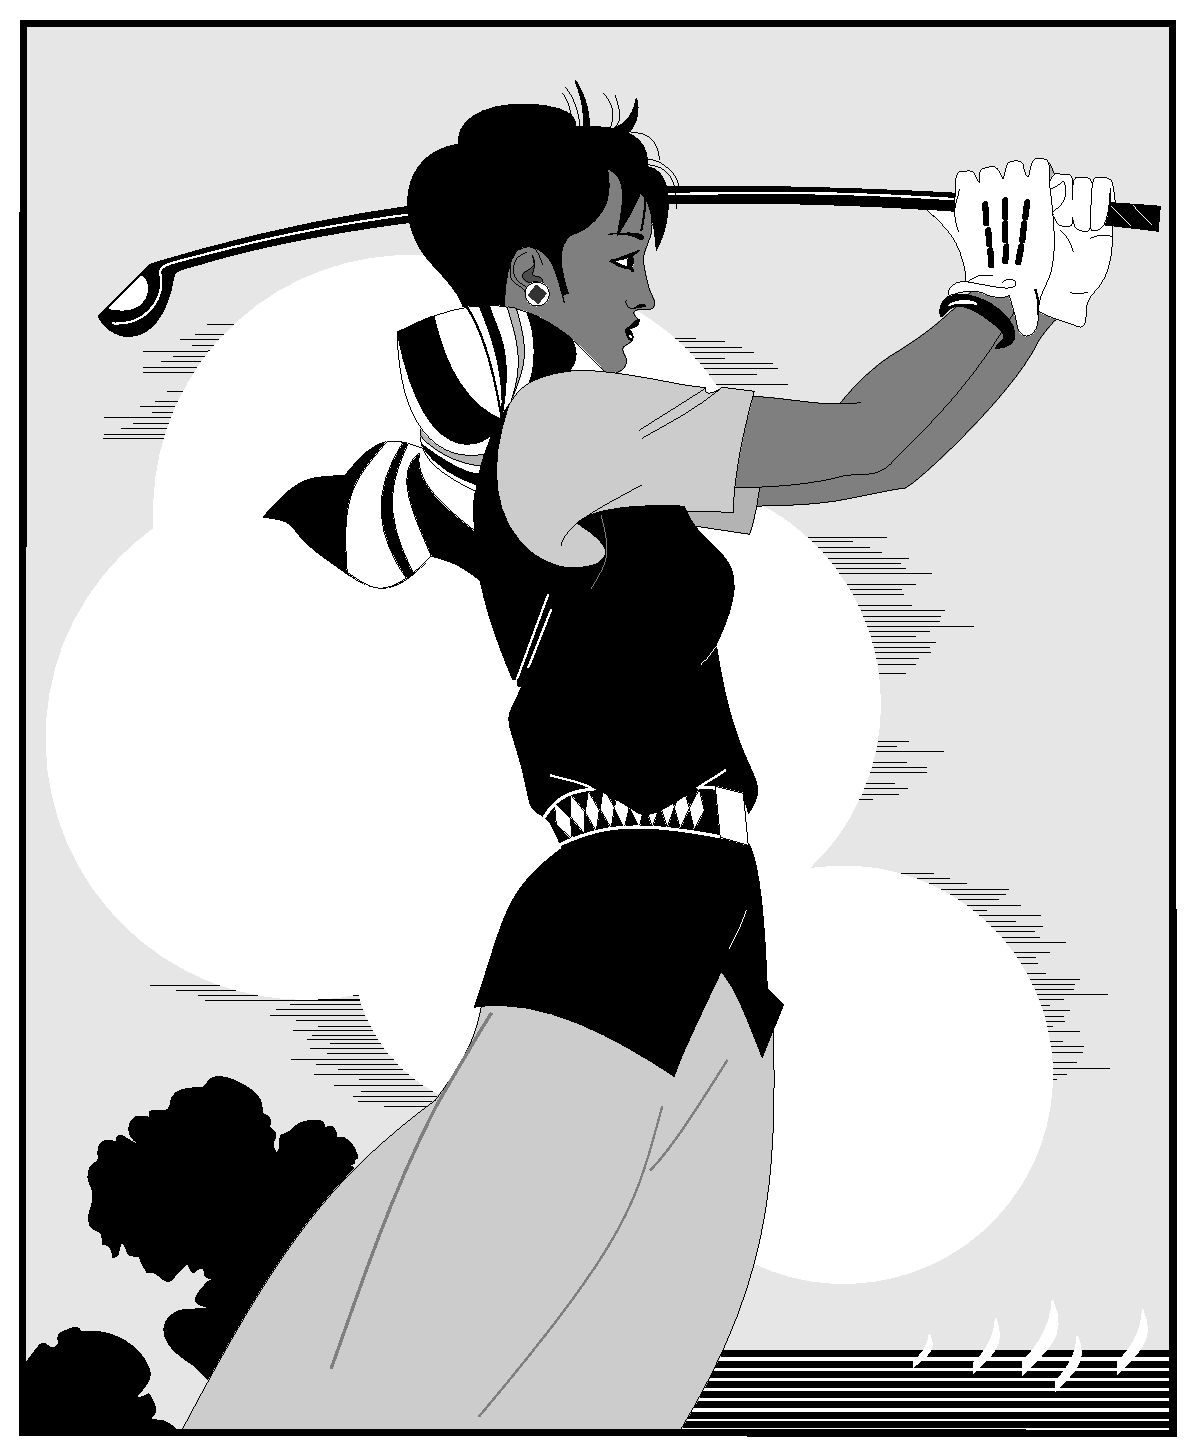
\includegraphics[width = 0.4\textwidth]{golfer}
\bicaption[golfer1]{}{打高尔夫球的人}{Fig.$\!$}{The person playing golf}\vspace{-1em}
\end{figure}

其插入图片的代码及其说明如下。
\vspace{1em}\noindent\hrule
\begin{lstlisting}
\begin{figure}[htbp]
\centering
\includegraphics[width=0.4\textwidth]{文件名(.eps)}
\bicaption[标签名(英文)]{}{中文标题}{Fig.$\!$}
          {English caption (首字母大写)}\vspace{-1em}
\end{figure}
\end{lstlisting}
\noindent\hrule
\begin{lstlisting}
figure环境的可选参数[htbp]表示浮动图形所放置的位置,h (here)表示当前位置,t (top)表示页芯顶部,b (bottom)表示页芯底部,p (page)表示单独一页。在word等软件中,图片通常插入到当前位置,如果当前页的剩余空间不够,图片将被移动到下一页,当前页就会出现很大的空白,其人工调整工作非常不便。由LaTeX提供的浮动图片功能,总是会按h->t->b->p的次序处理选项中的字母,自动调整图片的位置,大大减轻了工作量。
\centering命令将后续内容转换成每行皆居中的格式。
“\includegraphics”的可选参数用来设置图片插入文中的水平宽度,一般表示为正文宽度(\textwidth)的倍数。
\bicaption命令的使用需要调用ccaption宏包,它可以为图片或表格插入双语标题(博士学位论文要求),可选参数“标签名”为英文形式,一般不以图片或表格的数字顺序作为标签,而应包含一定的图片或表格信息,以便于文中引用(若图片、表格、公式、章节和参考文献等在文中出现的先后顺序发生了变化,其标注序号及其文中引用序号也会跟着发生变化,这一点是word等软件所不能做到的)。第4个参数中的“$\!$”表示-1/6个空铅宽度,这样可以缩小Fig.和Table与后面数字序号之间的水平距离。另外,图题或表题并不会因为分页而与图片或表格体分置于两页,章节等各级标题也不会置于某页的最底部,LaTeX系统会自动调整它们在正文中的位置,这也是word等软件所无法匹敌的。
注:硕士学位论文的图表只需要插入中文标题,因此需将\bicaption一句命令替换为如下两条命令(下同):
\caption{中文标题}
\label{标签名(英文)}
\vspace将产生一定高度的竖直空白,必选参数为负值表示将后续文字位置向上提升,参数值可自行调整。em为长度单位,相当于大写字母M的宽度。
引用方法:“见图~\ref{标签名(英文)}”、“如图~\ref{标签名(英文)}~所示”等。
\end{lstlisting}
\noindent\hrule\vspace{1em}
若需要将~2~张及以上的图片并排插入到一行中,则需要采用\verb|minipage|环境,如图~\ref{golfer2}~和图~\ref{golfer3}~所示。
\begin{figure}[htbp]
\centering
\begin{minipage}{0.4\textwidth}
\centering
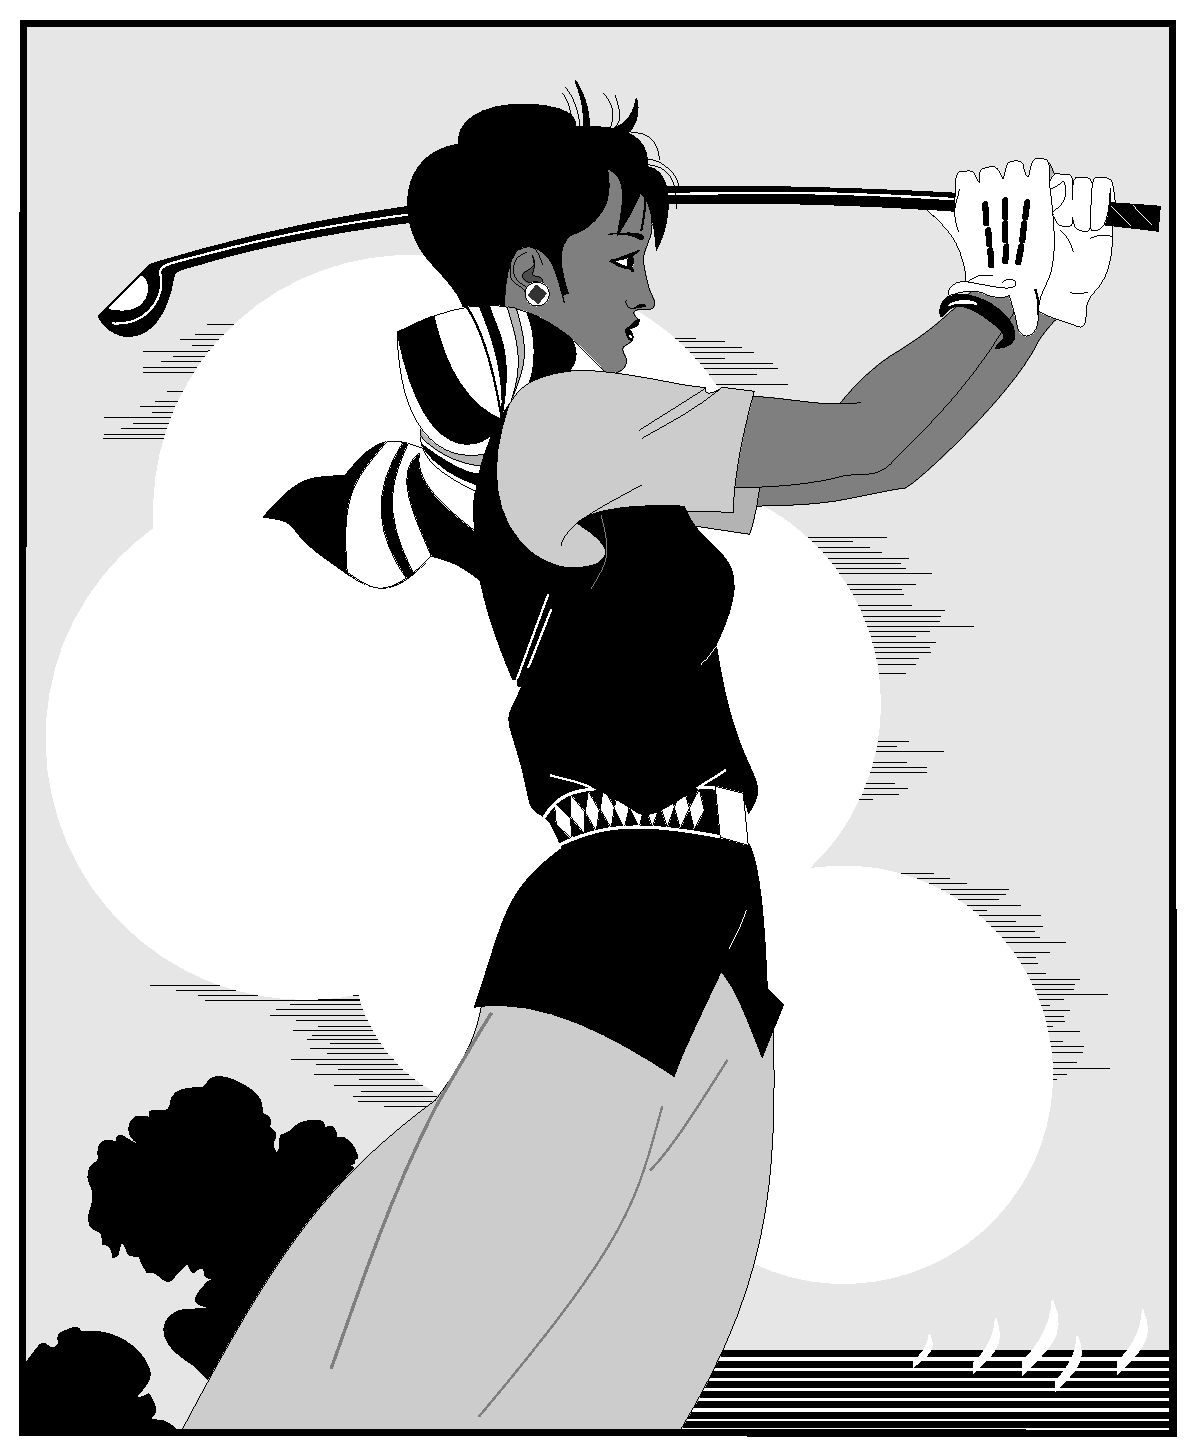
\includegraphics[width=\textwidth]{golfer}
\bicaption[golfer2]{}{打高尔夫球的人}{Fig.$\!$}{The person playing golf}
\end{minipage}
\begin{minipage}{0.4\textwidth}
\centering
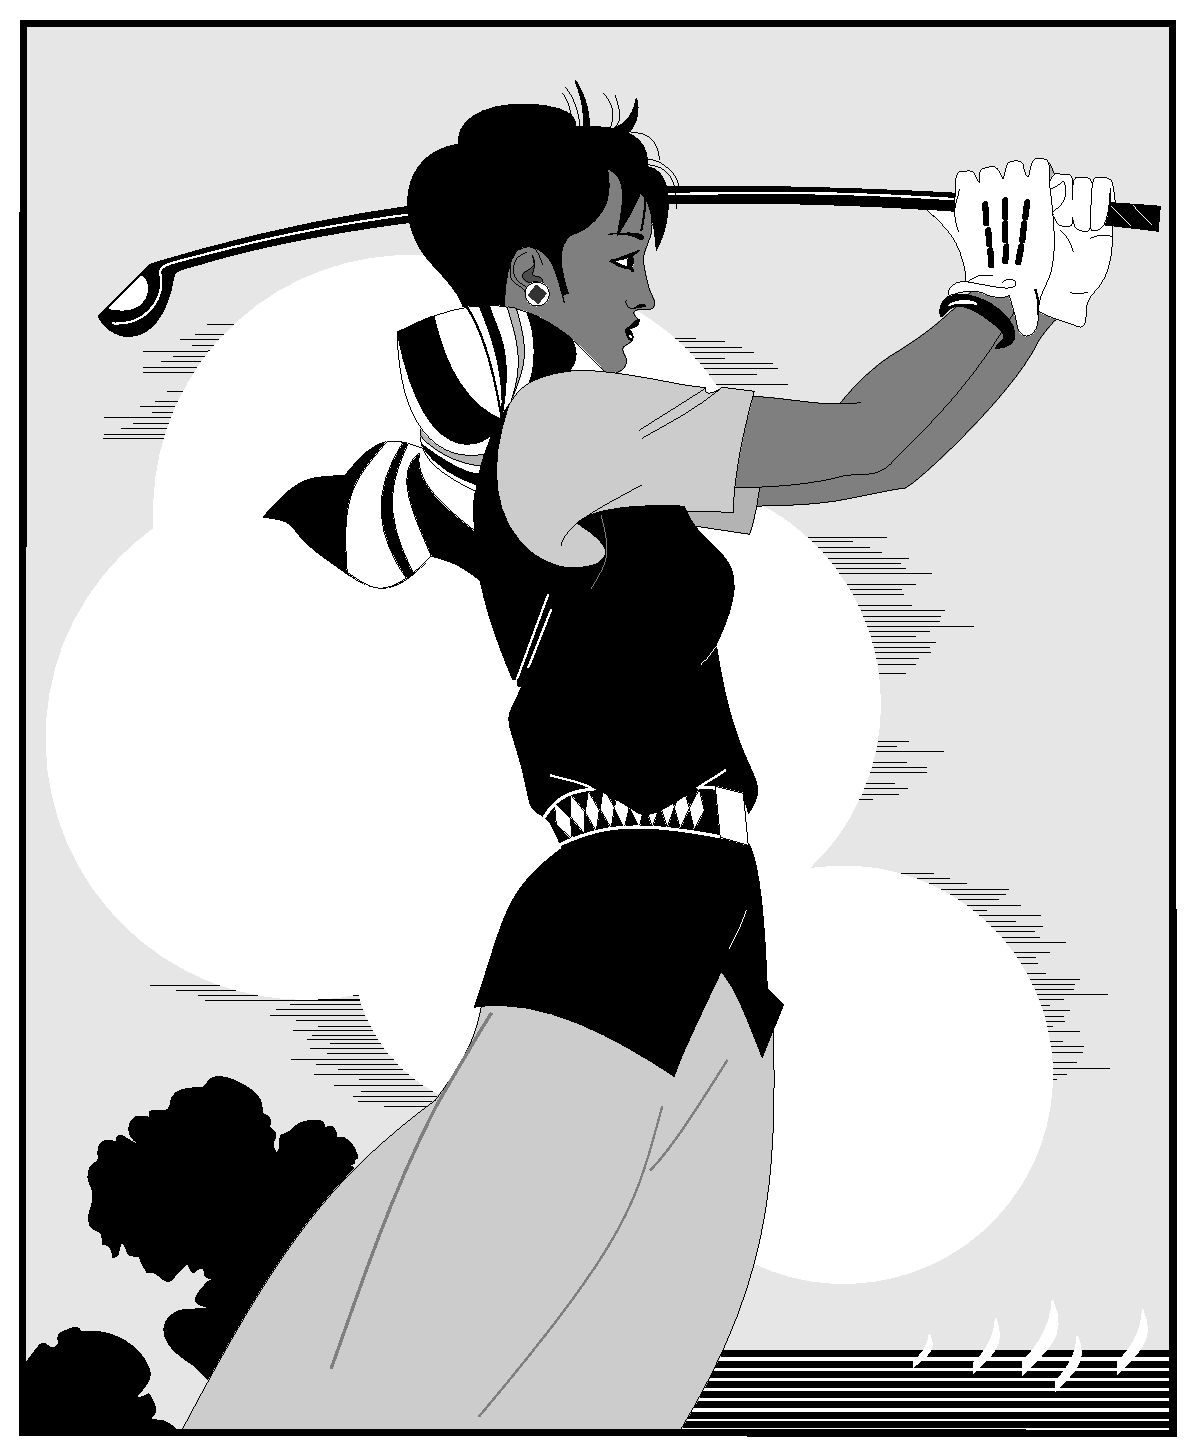
\includegraphics[width=\textwidth]{golfer}
\bicaption[golfer3]{}{打高尔夫球的人}{Fig.$\!$}{The person playing golf}
\end{minipage}\vspace{-1em}
\end{figure}

其代码如下所示。
\vspace{1em}\noindent\hrule
\begin{lstlisting}
\begin{figure}[htbp]
\centering
\begin{minipage}{0.4\textwidth}
\centering
\includegraphics[width=\textwidth]{文件名}
\bicaption[标签名]{}{中文标题}{Fig.$\!$}
          {English caption}
\end{minipage}
\begin{minipage}{0.4\textwidth}
\centering
\includegraphics[width=\textwidth]{文件名}
\bicaption[标签名]{}{中文标题}{Fig.$\!$}
          {English caption}
\end{minipage}\vspace{-1em}
\end{figure}
\end{lstlisting}
\noindent\hrule
\begin{lstlisting}
minipage环境的必选参数用来设置小页的宽度,若需要在一行中插入n个等宽图片,则每个小页的宽度应略小于(1/n)\textwidth。
\end{lstlisting}
\noindent\hrule

\BiSection{具有子图的图片插入方法}{The method of inserting figures with subfigures}

图中若含有子图时,需要调用~subfigure~宏包。博士学位论文规范要求不止总图的标题为中英文形式,其各个子图也应具有中英文形式的标题。
然而~ccaption~宏包却无法实现子图的中英文标题功能,这里采用对\verb|\subfigure|命令进行嵌套的方法来实现子图的中英文标题功能,如图~\ref{golfer4}~所示。

\begin{figure}[htbp]
\centering
\subfigure{\label{golfer41}}\addtocounter{subfigure}{-2}
\subfigure[The person playing golf]{\subfigure[打高尔夫球的人~1]{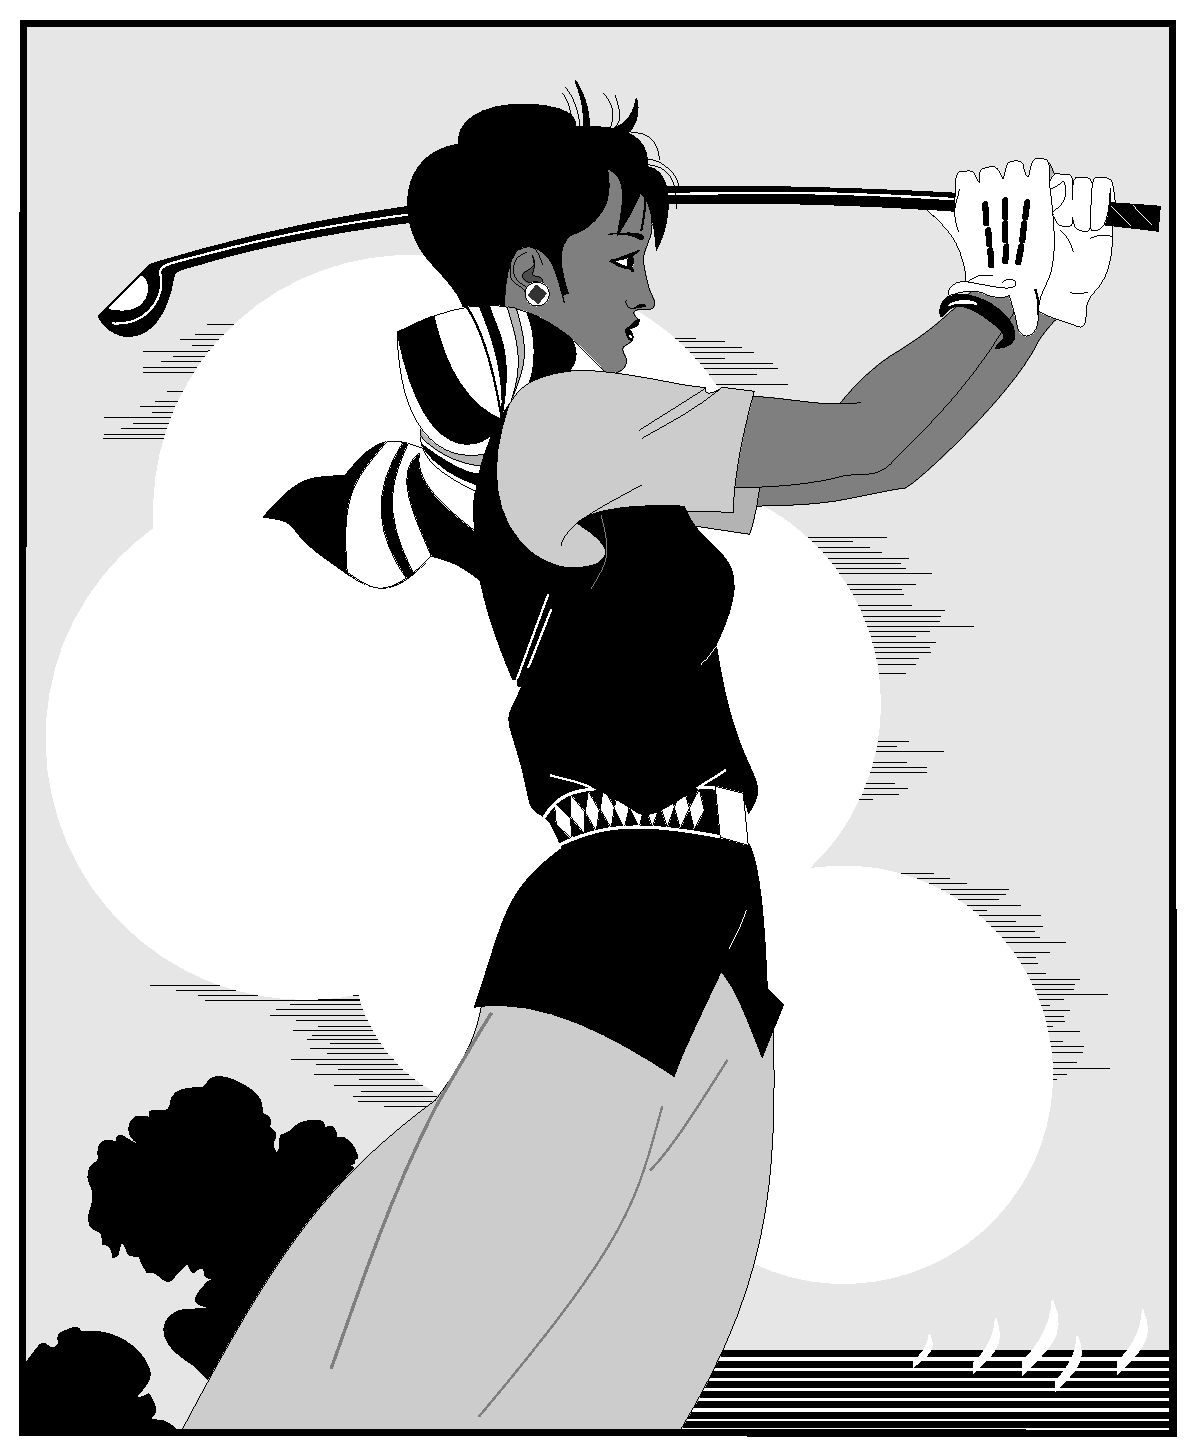
\includegraphics[width=0.4\textwidth]{golfer}}}
\subfigure{\label{golfer42}}\addtocounter{subfigure}{-2}
\subfigure[The person playing golf]{\subfigure[打高尔夫球的人~2]{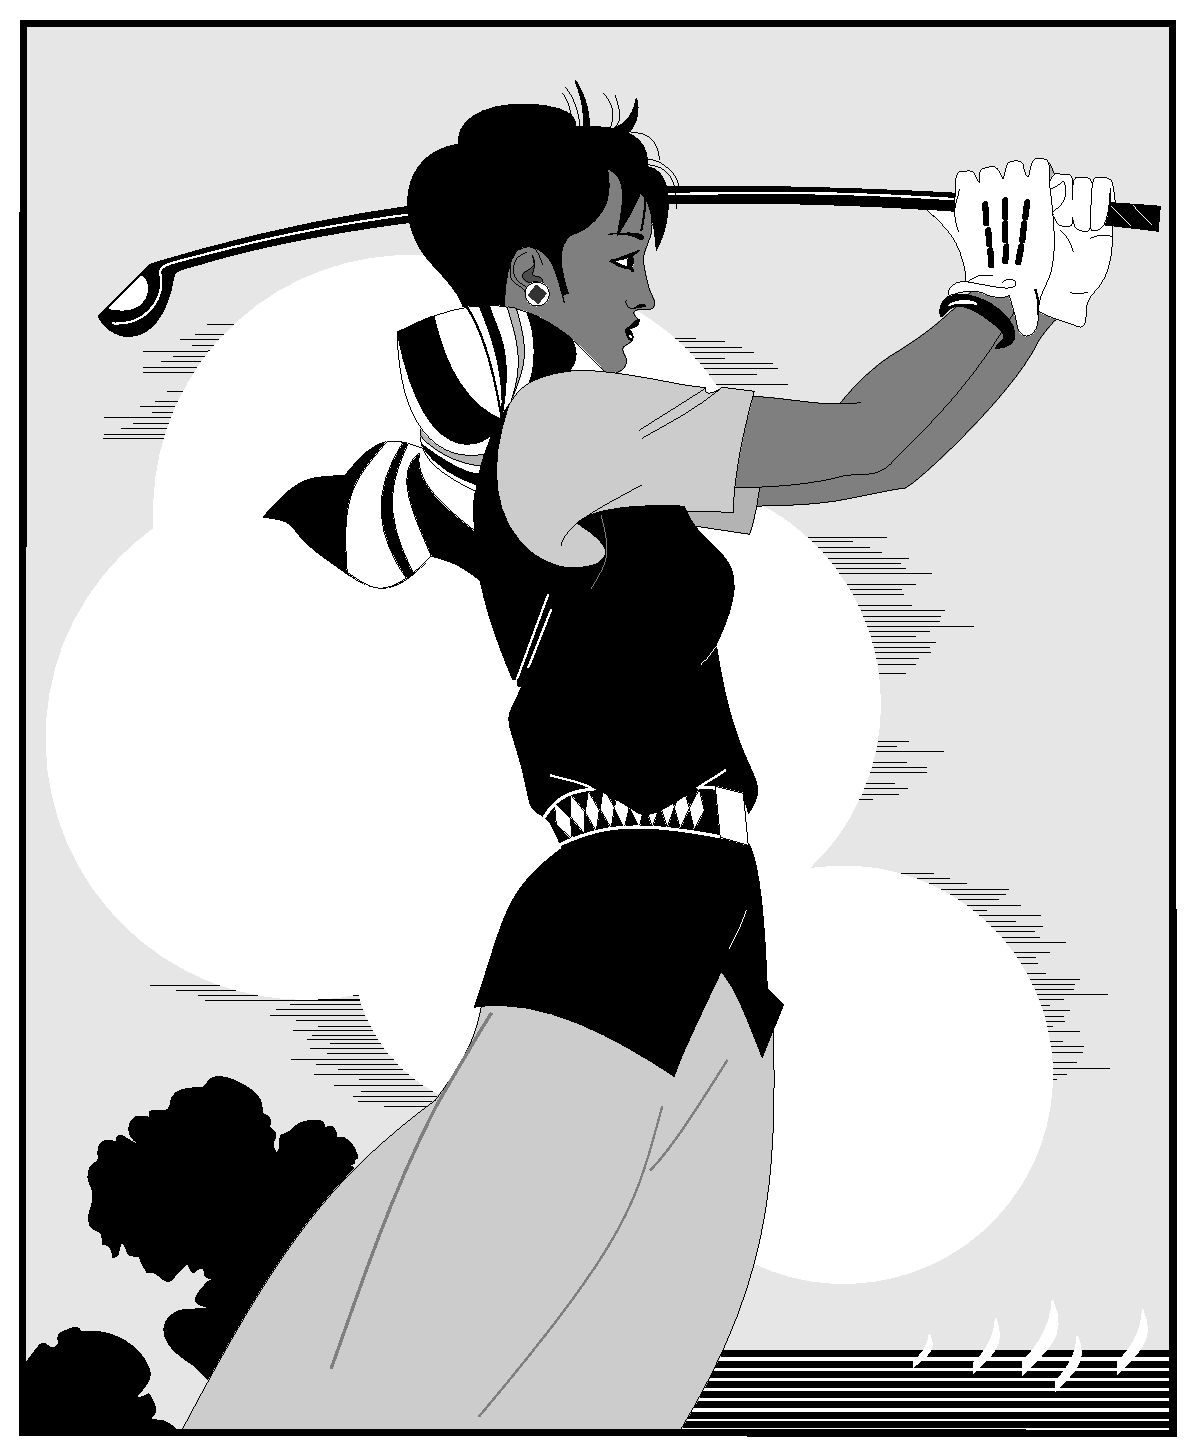
\includegraphics[width=0.4\textwidth]{golfer}}}
\bicaption[golfer4]{}{打高尔夫球的人}{Fig.$\!$}{The person playing golf}\vspace{-1em}
\end{figure}

其代码及其说明如下。
\vspace{1em}\noindent\hrule
\begin{lstlisting}
\begin{figure}[htbp]
\centering
\subfigure{\label{第1个子图标签名}}\addtocounter{subfigure}{-2}
\subfigure[The 1st subfigure caption]{\subfigure[第1个子图标题]
          {\includegraphics[width=0.4\textwidth]{文件名}}}
\subfigure{\label{第2个子图标签名}}\addtocounter{subfigure}{-2}
\subfigure[The 2nd subfigure caption]{\subfigure[第2个子图标题]
          {\includegraphics[width=0.4\textwidth]{文件名}}}
\bicaption[总标签名]{}{中文总标题}{Fig.$\!$}{The total caption}
\vspace{-1em}
\end{figure}
\end{lstlisting}
\noindent\hrule
\begin{lstlisting}
\addtocounter把指定的值加到计数器上,这里是对subfigure计数器进行减2操作。这是因为每插入1个子图,就调用3次\subfigure命令,第1次调用\subfigure命令用来生成紧随其后所插入子图的标签,而之后的双层嵌套调用\subfigure命令用来插入子图并生成该子图的中英文标题。因此,每插入1张子图,subfigure计数器的值就自动加3,为了使得子图的序号能每次加1,则需在每插入1张子图前手动把subfigure计数器的值减2。
\subfigure命令的双层嵌套使用可用来生成中英文标题,其内层\subfigure命令用来插入子图并生成中文标题,外层\subfigure命令将插入的子图和中文标题作为一个整体,生成这个整体的英文标题,因此英文标题会置于中文标题的下面。
硕士学位论文只需要中文标题,其代码如下:
\begin{figure}[htbp]
\centering
\subfigure[第1个子图标题\label{第1个子图标签名}]
          {\includegraphics[width=0.4\textwidth]{文件名}}
\subfigure[第2个子图标题\label{第2个子图标签名}]
          {\includegraphics[width=0.4\textwidth]{文件名}}
\caption{中文总标题}\label{总标签名}
\vspace{-1em}
\end{figure}
引用方法:总图的引用方法同本章第1节,子图的引用方法用\ref{第n个子图标签名}来代替。
\end{lstlisting}
\noindent\hrule\vspace{1em}

子图的引用示例:如图~\ref{golfer41}~和图~\ref{golfer42}~所示。

若想获得插图方法的更多信息,请参见网络上的~\href{ftp://ftp.tex.ac.uk/tex-archive/info/epslatex.pdf}{Using Imported Graphics in \LaTeX and pdf\LaTeX}~文档。 

%% !Mode:: "TeX:UTF-8" 

\BiChapter{表格的绘制方法}{Methods of drawing tables}
\BiSection{研究生院的绘表规范}{Tables drawing standard from graduate school}

表应有自明性。表格不加左、右边线。表的编排建议采用国际通行的三线表。表中文字用宋体~5~号字。

每个表格均应有表题(由表序和表名组成)。表序一般按章编排,如第~1~章第一个插表的序号为“表~1-1”等。表序与表名之间空一格,
表名中不允许使用标点符号,表名后不加标点。表题置于表上,硕士学位论文只用中文,博士学位论文用中、英文两种文字居中排写,
中文在上,要求中文用宋体~5~号字,英文用新罗马字体~5~号字。

表头设计应简单明了,尽量不用斜线。表头中可采用化学符号或物理量符号。

全表如用同一单位,则将单位符号移至表头右上角,加圆括号。
表中数据应准确无误,书写清楚。数字空缺的格内加横线“-”(占~2~个数字宽度)。表内文字或数字上、下或左、右相同时,
采用通栏处理方式,不允许用“〃”、“同上”之类的写法。

表内文字说明,起行空一格、转行顶格、句末不加标点。

如某个表需要转页接排,在随后的各页上应重复表的编号。编号后加“(续表)”,表题可省略。续表应重复表头。

\BiSection{普通表格的绘制方法}{Methods of drawing normal tables}

表格应具有三线表格式,因此需要调用~booktabs~宏包,其标准格式如表~\ref{table1}~所示。
\begin{table}[htbp]
\bicaption[table1]{}{符合研究生院绘图规范的表格}{Table$\!$}{Table in agreement of the standard from graduate school}
\vspace{0.5em}\centering\wuhao
\begin{tabular}{ccccc}
\toprule[1.5pt]
$D$(in) & $P_u$(lbs) & $u_u$(in) & $\beta$ & $G_f$(psi.in)\\
\midrule[1pt]
 5 & 269.8 & 0.000674 & 1.79 & 0.04089\\
10 & 421.0 & 0.001035 & 3.59 & 0.04089\\
20 & 640.2 & 0.001565 & 7.18 & 0.04089\\
\bottomrule[1.5pt]
\end{tabular}
\end{table}

其绘制表格的代码及其说明如下。
\vspace{1em}\noindent\hrule
\begin{lstlisting}
\begin{table}[htbp]
\bicaption[标签名]{}{中文标题}{Table$\!$}{English caption}
\vspace{0.5em}\centering\wuhao
\begin{tabular}{cc...c}
\toprule[1.5pt]
表头第1个格   & 表头第2个格   & ... & 表头第n个格  \\
\midrule[1pt]
表中数据(1,1) & 表中数据(1,2) & ... & 表中数据(1,n)\\
表中数据(2,1) & 表中数据(2,2) & ... & 表中数据(2,n)\\
...................................................\\
表中数据(m,1) & 表中数据(m,2) & ... & 表中数据(m,n)\\
\bottomrule[1.5pt]
\end{tabular}
\end{table}
\end{lstlisting}
\noindent\hrule
\begin{lstlisting}
table环境是一个将表格嵌入文本的浮动环境。
\wuhao命令将表格的字号设置为五号字(10.5pt),在绘制表格结束退出时,不需要将字号再改回为\xiaosi,正文字号默认为小四号字(12pt)。
tabular环境的必选参数由每列对应一个格式字符所组成:c表示居中,l表示左对齐,r表示右对齐,其总个数应与表的列数相同。此外,@{文本}可以出现在任意两个上述的列格式之间,其中的文本将被插入每一行的同一位置。表格的各行以\\分隔,同一行的各列则以&分隔。
\toprule、\midrule和\bottomrule三个命令是由booktabs宏包提供的,其中\toprule和\bottomrule分别用来绘制表格的第一条(表格最顶部)和第三条(表格最底部)水平线,\midrule用来绘制第二条(表头之下)水平线,且第一条和第三条水平线的线宽为1.5pt,第二条水平线的线宽为1pt。
引用方法:“如表~\ref{标签名}~所示”。
\end{lstlisting}
\noindent\hrule

\BiSection{长表格的绘制方法}{Methods of drawing long tables}

长表格是当表格在当前页排不下而需要转页接排的情况下所采用的一种表格环境。若长表格仍按照普通表格的绘制方法来获得,
其所使用的\verb|table|浮动环境无法实现表格的换页接排功能,表格下方过长部分会排在表格第1页的页脚以下。为了能够实现长表格的转页接排功能,
需要调用~longtable~宏包,由于长表格是跨页的文本内容,因此只需要单独的\verb|longtable|环境,所绘制的长表格的格式如表~\ref{table2}~所示。

此长表格~\ref{table2}~第~2~页的标题“编号(续表)”和表头是通过代码自动添加上去的,无需人工添加,若表格在页面中的竖直位置发生了变化,长表格在第~2~页
及之后各页的标题和表头位置能够始终处于各页的最顶部,也无需人工调整,\LaTeX~系统的这一优点是~word~等软件所无法比拟的。

\wuhao\begin{longtable}{ccc}
\longbionenumcaption{}{中国省级行政单位一览\label{table2}}{Table$\!$}{}{Overview of the provincial administrative unit of China} \vspace{0.5em}\\
\toprule[1.5pt] 名称 & 简称 & 省会或首府  \\ \midrule[1pt]
\endfirsthead
\multicolumn{3}{r}{表~\thetable(续表)}\vspace{0.5em}\\
\toprule[1.5pt] 名称 & 简称 & 省会或首府  \\ \midrule[1pt]
\endhead
\bottomrule[1.5pt]
\endfoot
北京市 & 京 & 北京\\
天津市 & 津 & 天津\\
河北省 & 冀 & 石家庄市\\
山西省 & 晋 & 太原市\\
内蒙古自治区 & 蒙 & 呼和浩特市\\
辽宁省 & 辽 & 沈阳市\\
吉林省 & 吉 & 长春市\\
黑龙江省 & 黑 & 哈尔滨市\\
上海市 & 沪/申 & 上海\\
江苏省 & 苏 & 南京市\\
浙江省 & 浙 & 杭州市\\
安徽省 & 皖 & 合肥市\\
福建省 & 闽 & 福州市\\
江西省 & 赣 & 南昌市\\
山东省 & 鲁 & 济南市\\
河南省 & 豫 & 郑州市\\
湖北省 & 鄂 & 武汉市\\
湖南省 & 湘 & 长沙市\\
广东省 & 粤 & 广州市\\
广西壮族自治区 & 桂 & 南宁市\\
海南省 & 琼 & 海口市\\
重庆市 & 渝 & 重庆\\
四川省 & 川/蜀 & 成都市\\
贵州省 & 黔/贵 & 贵阳市\\
云南省 & 云/滇 & 昆明市\\
西藏自治区 & 藏 & 拉萨市\\
陕西省 & 陕/秦 & 西安市\\
甘肃省 & 甘/陇 & 兰州市\\
青海省 & 青 & 西宁市\\
宁夏回族自治区 & 宁 & 银川市\\
新疆维吾尔自治区 & 新 & 乌鲁木齐市\\
香港特别行政区 & 港 & 香港\\
澳门特别行政区 & 澳 & 澳门\\
台湾省 & 台 & 台北市\\
\end{longtable}\xiaosi

绘制长表格的代码及其说明如下。
\vspace{1em}\noindent\hrule
\begin{lstlisting}

\wuhao\begin{longtable}{cc...c}
\longbionenumcaption{}{中文标题\label{标签名}}{Table$\!$}
                    {}{English caption}\vspace{0.5em}\\
\toprule[1.5pt] 表头第1个格 & 表头第2个格 & ... & 表头第n个格\\ \midrule[1pt]
\endfirsthead
\multicolumn{n}{r}{表~\thetable(续表)}\vspace{0.5em}\\
\toprule[1.5pt] 表头第1个格 & 表头第2个格 & ... & 表头第n个格\\ \midrule[1pt]
\endhead
\bottomrule[1.5pt]
\endfoot
表中数据(1,1) & 表中数据(1,2) & ... & 表中数据(1,n)\\
表中数据(2,1) & 表中数据(2,2) & ... & 表中数据(2,n)\\
...................................................\\
表中数据(m,1) & 表中数据(m,2) & ... & 表中数据(m,n)\\
\end{longtable}\xiaosi
\end{lstlisting}
\noindent\hrule
\begin{lstlisting}
在绘制长表格的前面留出一个空白行,并在第2行的一开始全局定义长表格的字号为五号字,这样能够保证长表格之前段落的行距保持不变。在绘制长表格结束后,需要\xiaosi命令重新将字号改为小四号字。
长表格的中英文标题是通过ccaption宏包的\longbionenumcaption命令得到的。
\endhead之前的文字描述的是第2页及其之后各页的标题或表头;\endfirsthead之前的文字描述的是第1页的标题和表头,若无此命令,则第1页的表头和标题由\endhead命令确定;同理,\endfoot之前的文字描述的是除最后一页之外每页的表格底部内容;\endlastfoot之前的文字描述的是最后一页的表格底部内容,若无此命令,则最后一页的表格底部内容由\endfoot命令确定;由于规范中长表格每页底部内容均相同(水平粗线),因此模板中没有用到\endlastfoot命令。
注:硕士学位论文的长表格只需要插入中文标题,因此需将\longbionenumcaption一句命令替换为如下两条命令 :
\caption{中文标题}
\label{标签名}
\end{lstlisting}
\noindent\hrule

\BiSection{列宽可调表格的绘制方法}{Methods of drawing tables with adjustable-width columns}
论文中能用到列宽可调表格的情况共有两种,一种是当插入的表格某一单元格内容过长以至于一行放不下的情况,
另一种是当对公式中首次出现的物理量符号进行注释的情况,这两种情况都需要调用~tabularx~宏包。下面将分别对这两种情况下可调表格的绘制方法进行阐述。
\BiSubsection{表格内某单元格内容过长的情况}{The condition when the contents in some cells of tables are too long}
首先给出这种情况下的一个例子如表~\ref{table3}~所示。
\begin{table}[htbp]
  \centering
\bicaption[table3]{}{最小的三个正整数的英文表示法}{Table$\!$}{The English construction of the smallest three positive integral numbers}\vspace{0.5em}\wuhao
\begin{tabularx}{0.7\textwidth}{llX}
\toprule[1.5pt]
Value & Name & Alternate names, and names for sets of the given size\\\midrule[1pt]
1 & One & ace, single, singleton, unary, unit, unity\\
2 & Two & binary, brace, couple, couplet, distich, deuce, double, doubleton, duad, duality, duet, duo, dyad, pair, snake eyes, span, twain, twosome, yoke\\
3 & Three & deuce-ace, leash, set, tercet, ternary, ternion, terzetto, threesome, tierce, trey, triad, trine, trinity, trio, triplet, troika, hat-trick\\\bottomrule[1.5pt]
\end{tabularx}
\end{table}

绘制这种表格的代码及其说明如下。
\vspace{1em}\noindent\hrule
\begin{lstlisting}
\begin{table}[htbp]
\bicaption[标签名]{}{中文标题}{Table$\!$}{English caption}
\vspace{0.5em}\wuhao
\begin{tabularx}{\textwidth}{l...X...l}
\toprule[1.5pt]
表头第1个格   & ... & 表头第X个格   & ... & 表头第n个格  \\
\midrule[1pt]
表中数据(1,1) & ... & 表中数据(1,X) & ... & 表中数据(1,n)\\
表中数据(2,1) & ... & 表中数据(2,X) & ... & 表中数据(2,n)\\
.........................................................\\
表中数据(m,1) & ... & 表中数据(m,X) & ... & 表中数据(m,n)\\
\bottomrule[1.5pt]
\end{tabularx}
\end{table}
\end{lstlisting}
\noindent\hrule

\begin{lstlisting}

tabularx环境共有两个必选参数:第1个参数用来确定表格的总宽度,这里取为排版表格能达到的最大宽度——正文宽度\textwidth;第2个参数用来确定每列格式,其中标为X的项表示该列的宽度可调,其宽度值由表格总宽度确定。
标为X的列一般选为单元格内容过长而无法置于一行的列,这样使得该列内容能够根据表格总宽度自动分行。若列格式中存在不止一个X项,则这些标为X的列的列宽相同,因此,一般不将内容较短的列设为X。
标为X的列均为左对齐,因此其余列一般选为l(左对齐),这样可使得表格美观,但也可以选为c或r。

\end{lstlisting}

\noindent\hrule

\BiSubsection{对物理量符号进行注释的情况}{The condition when physical symbols need to be annotated}

为使得对公式中物理量符号注释的转行与破折号“———”后第一个字对齐,此处最好采用表格环境。此表格无任何线条,左对齐,
且在破折号处对齐,一共有“式中”二字、物理量符号和注释三列,表格的总宽度可选为文本宽度,因此应该采用\verb|tabularx|环境。
由\verb|tabularx|环境生成的对公式中物理量符号进行注释的公式如式(\ref{eq:1})所示。

\begin{equation}\label{eq:1}
\ddot{\boldsymbol{\rho}}-\frac{\mu}{R_{t}^{3}}\left(3\mathbf{R_{t}}\frac{\mathbf{R_{t}\rho}}{R_{t}^{2}}-\boldsymbol{\rho}\right)=\mathbf{a}
\end{equation}
\begin{tabularx}{\textwidth}{@{}l@{\quad}r@{———}X@{}}
式中& $\boldsymbol{\rho}$ &追踪飞行器与目标飞行器之间的相对位置矢量;\\
&  $\boldsymbol{\ddot{\rho}}$&追踪飞行器与目标飞行器之间的相对加速度;\\
&  $\mathbf{a}$   &推力所产生的加速度;\\
&  $\mathbf{R_t}$ & 目标飞行器在惯性坐标系中的位置矢量;\\
&  $\omega_{t}$ & 目标飞行器的轨道角速度;\\
&  $\mathbf{g}$ & 重力加速度,$=\frac{\mu}{R_{t}^{3}}\left(
3\mathbf{R_{t}}\frac{\mathbf{R_{t}\rho}}{R_{t}^{2}}-\boldsymbol{\rho}\right)=\omega_{t}^{2}\frac{R_{t}}{p}\left(
3\mathbf{R_{t}}\frac{\mathbf{R_{t}\rho}}{R_{t}^{2}}-\boldsymbol{\rho}\right)$,这里~$p$~是目标飞行器的轨道半通径。
\end{tabularx}\vspace{\wordsep}

其中生成注释部分的代码及其说明如下。
\vspace{1em}\noindent\hrule
\begin{lstlisting}
\begin{tabularx}{\textwidth}{@{}l@{\quad}r@{— — —}X@{}}
式中 & symbol-1 & symbol-1的注释内容;\\
     & symbol-2 & symbol-2的注释内容;\\
     .............................;\\
     & symbol-m & symbol-m的注释内容。
\end{tabularx}\vspace{\wordsep}
\end{lstlisting}
\noindent\hrule
\begin{lstlisting}
tabularx环境的第1个参数选为正文宽度,第2个参数里面各个符号的意义为:
    第1个@{}表示在“式中”二字左侧不插入任何文本,“式中”二字能够在正文中左对齐,若无此项,则“式中”二字左侧会留出一定的空白;
    @{\quad}表示在“式中”和物理量符号间插入一个空铅宽度的空白;
    @{— — —}实现插入破折号的功能,它由三个1/2的中文破折号构成;
    第2个@{}表示在注释内容靠近正文右边界的地方能够实现右对齐。
\end{lstlisting}
\noindent\hrule\vspace{1em}
由此方法生成的注释内容应紧邻待注释公式并置于其下方,因此不能将代码放入\verb|table|浮动环境中。但此方法不能实现自动转页接排,
可能会在当前页剩余空间不够时,全部移动到下一页而导致当前页出现很大空白。因此在需要转页处理时,还请您手动将需要转页的代码放入一个
新的\verb|tabularx|环境中,将原来的一个\verb|tabularx|环境拆分为两个\verb|tabularx|环境。

若想获得绘制表格的更多信息,请参见网络上的~\href{http://www.tug.org/pracjourn/2007-1/mori/}{Tables in \LaTeXe: Packages and Methods}~文档。 

%% !Mode:: "TeX:UTF-8" 

\BiChapter{数学公式的输入方法}{Input methods of equations}
\BiSection{研究生院的公式规范}{Equations typesetting standard from graduate school}
论文中的公式应另起行,原则上应居中书写,与周围文字留有足够的空间区分开。
若公式前有文字(如“解”、“假定”等),文字空两格写,公式仍居中写。公式末不加标点。

公式应标注序号,并将序号置于括号内。 公式序号按章编排,如第~1~章第一个公式序号为“(1-1)”。公式的序号右端对齐。

公式较长时最好在等号“=”处转行,如难实现,则可在~$+$、$-$、$\times$、$\div$~运算符号处转行,转行时运算符号仅书写于转行式前,不重复书写。

文中引用公式时,一般用“见式~(1-1)”或“由公式~(1-1)”。

公式中用斜线表示“除”的关系时应采用括号,以免含糊不清,如~$a/(b\cos x)$。通常“乘”的关系在前,如~$a\cos x/b$而不写成~$(a/b)\cos x$。

不能用文字形式表示等式,如:$\textnormal{刚度}=\frac{{\textnormal{受力}}}{{\textnormal{受力方向的位移}}}$。

\textbf{对于数学公式的输入方法,网络上有一个比较全面权威的文档~\href{http://tug.ctan.org/cgi-bin/ctanPackageInformation.py?id=voss-mathmode}{Math mode}~请大家事先大概浏览一下。下面将对学位论文中主要用到的数学公式排版形式进行阐述。}

\BiSection{生成~\LaTeX~数学公式的两种方法}{Two methods of generating \LaTeX equations}
对于先前没有接触过~\LaTeX~的人来说,编写~\LaTeX~数学公式是一件很繁琐的事,尤其是对复杂的数学公式来说,更可以说是一件难以完成的任务。
实际上,生成~\LaTeX~数学公式有两种较为简便的方法,一种是基于~MathType~数学公式编辑器的方法,另一种是基于~MATLAB~商业数学软件的方法,
下面将分别对这两种数学公式的生成方法作一下简单介绍。
\BiSubsection{基于~MathType~软件的数学公式生成方法}{Generating method of equations based on MathType}
MathType~是一款功能强大的数学公式编辑器软件,能够用来在文本环境中插入~Windows OLE~图形格式的复杂数学公式,所以应用比较普遍。但此软件只有~30~天的试用期,之后若再继续使用则需要付费购买才行。网络上有很多破解版的~MathType~软件可供下载免费使用,
笔者推荐下载安装版本号在~6.5~之上的中文破解版。

在安装好~MathType~之后,若在输入窗口中编写数学公式,复制到剪贴板上的仍然是图形格式的对象。
若希望得到可插入到~\LaTeX~编辑器中的文本格式对象,则需要对~MathType~软件做一下简单的设置:在~MathType~最上排的按钮中依次选择“参数选项
$\to$转换”,在弹出的对话窗中选中“转换到其它语言(文字):”,在转换下拉框中选择“Tex~--~--~LaTeX 2.09 and later”,并将对话框最下方的两个复选框全部勾掉,点击确定,这样,再从输入窗口中复制出来的对象就是文本格式的了,就可以直接将其粘贴到~\LaTeX~
编辑器中了。按照这种方法生成的数学公式两端分别有标记\verb|\[|和标记\verb|\]|,在这两个标记之间才是真正的数学公式代码。

若希望从~MathType~输入窗口中复制出来的对象为图形格式,则只需再选中“公示对象(Windows OLE~图形)”即可。

\BiSubsection{基于~MATLAB~软件的数学公式生成方法}{Generating method of equations based on Matlab}
MATLAB~是矩阵实验室(Matrix Laboratory)的简称,是美国~MathWorks~公司出品的商业数学软件。它是当今科研领域最常用的应用软件之一,
具有强大的矩阵计算、符号运算和数据可视化功能,是一种简单易用、可扩展的系统开发环境和平台。

MATLAB~中提供了一个~latex~函数,它可将符号表达式转化为~\LaTeX~数学公式的形式。其语法形式为~latex(s),其中,~s~为符号表达式,
之后再将~latex~函数的运算结果直接粘贴到~\LaTeX~编辑器中。从~\LaTeX~数学公式中可以发现,其中可能包含如下符号组合:
\begin{lstlisting}
\qquad=两个空铅(quad)宽度
\quad=一个空铅宽度
\;=5/18空铅宽度
\:=4/18空铅宽度
\,=3/18空铅宽度
\!=-3/18空铅宽度
\ =一个空格
\end{lstlisting}
所以最好将上述符号组合从数学公式中删除,从而使数学公式显得匀称美观。

对于~word~等软件的使用者来说,在我们通过~MATLAB~运算得到符号表达式形式的运算结果时,在~word~中插入运算结果需要借助于~MathType~软件,
通过在~MathType~中输入和~MATLAB~运算结果相对应的数学表达形式,之后再将~MathType~数学表达式转换为图形格式粘贴到~word~中。实际上,
也可以将~MATLAB~中采用~latex~函数运行的结果直接粘贴到~MathType~中,再继续上述步骤,这样可以大大节省输入公式所需要的时间。
此方法在~MathType~6.5c~上验证通过,若您粘入到~MathType~中的仍然为从~MATLAB~中导入的代码,请您更新~MathType~软件。

\BiSection{数学字体}{Math fonts}
在数学模式下,常用的数学字体命令有如下几种:
\begin{lstlisting}
\mathnormal或无命令 用数学字体打印文本;
\mathit             用斜体(\itshape)打印文本;
\mathbf             用粗体(\bfseries)打印文本;
\mathrm             用罗马体(\rmfamily)打印文本;
\mathsf             用无衬线字体(\sffamily)打印文本;
\mathtt             用打印机字体(\ttfamily)打印文本;
\mathcal            用书写体打印文本。
\end{lstlisting}
在学位论文撰写中,只需要用到上面提到的~\verb|\mathit|、\verb|\mathbf|~和~\verb|\mathrm|~命令。若要得到~Times New Roman~的数学字体,则需要调用~txfonts~宏包(此宏包实际上采用的是~Nimbus Roman No9 L~字体,
它是开源系统中使用的免费字体,其字符字体与~Times New Roman~字体几乎完全相同)。表~\ref{table:fonts}~中分别列出了得到阿拉伯数字、拉丁字母和希腊字母
各种数学字体的命令。
\begin{table}[htbp]
\bicaption[table:fonts]{}{常用数学字体命令一览}{Table$\!$}{Summary of common commands for setting math fonts}
\vspace{0.5em}\centering\wuhao

\begin{tabular}{llll}
\toprule
 & 阿拉伯数字\&大写希腊字母 & 大小写拉丁字母 & 小写希腊字母  \\
\midrule
斜体 & \verb|\mathit{}| & \verb|无命令| & \verb|无命令|\\
粗斜体 & \verb|\boldsymbol{\mathit{}}| & \verb|\boldsymbol{}| & \verb|\boldsymbol{}|\\
直立体 & \verb|无命令| & \verb|\mathrm{}| & \verb|字母后加up|\\
粗体 & \verb|\mathbf{}或\boldsymbol{}| & \verb|\mathbf{}| & \verb|\boldsymbol{字母后加up}|\\
\bottomrule
\end{tabular}
\end{table}

\noindent 下面列出了一些应采用直立数学字体的数学常数和数学符号。

\vspace{-0.5em}\begin{center}\begin{tabularx}{0.7\textwidth}{XX}
$\mathrm{d}$、 $\mathrm{D}$、 $\mathrm{p}$~———微分算子 & $\mathrm{e}$~———自然对数之底数\\
$\mathrm{i}$、 $\mathrm{j}$~———虚数单位 & $\pi$———圆周率\\
\end{tabularx}\end{center}

\BiSection{行内公式}{Inline mode equations}
出现在正文一行之内的公式称为行内公式,例如~$f(x)=\int_{a}^{b}\frac{\sin{x}}{x}\mathrm{d}x$。对于非矩阵和非多行形式的行内公式,一般不会使得行距发生变化,而~word~等软件却会根据行内公式的竖直距离而自动调节行距,如图~\ref{hangju}~所示。
\begin{figure}[htbp]
\centering
\subfigure{\label{latex}}\addtocounter{subfigure}{-2}
\subfigure[Inline mode equation derived from \LaTeX system]{\subfigure[由~\LaTeX~系统生成的行内公式]
          {\fbox{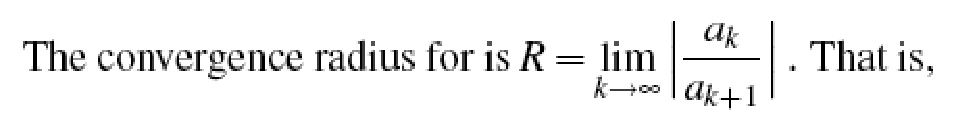
\includegraphics[width=0.55\textwidth]{latex}}}}
\subfigure{\label{word}}\addtocounter{subfigure}{-2}
\subfigure[Inline mode equation displayed as .doc format file derived from word software]{\subfigure[由~word软件生成的~.doc~格式行内公式]
          {\fbox{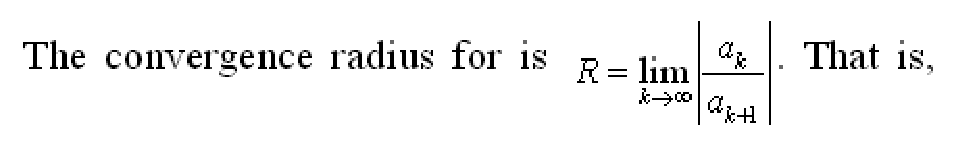
\includegraphics[width=0.55\textwidth]{word}}}}
\subfigure{\label{pdf}}\addtocounter{subfigure}{-2}
\subfigure[Inline mode equation displayed as .pdf format file derived from word software]{\subfigure[由~word软件生成的~.pdf~格式行内公式]
          {\fbox{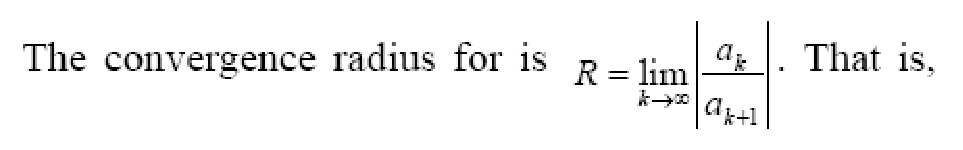
\includegraphics[width=0.55\textwidth]{pdf}}}}
\bicaption[hangju]{}{由~\LaTeX~和~word~生成的~3~种行内公式屏显效果}{Fig.$\!$}{Three kinds of inline mode equation displayed effects derived from \LaTeX and word}
\vspace{-1em}
\end{figure}
这三幅图分别为~\LaTeX~和~word~生成的行内公式屏显效果,从图中可看出,在~\LaTeX~文本含有公式的行内,在正文与公式之间对接工整,行距不变;而在~word~文本含有公式的行内,在正文与公式之间对接不齐,行距变大。因此从这一点来说,
\LaTeX~系统在数学公式的排版上具有很大优势。

\LaTeX~提供的行内公式最简单、最有效的方法是采用~\TeX~本来的标记———开始和结束标记都写作~\$,例如本节开始的例子可由下面的输入得到。
\verb|$f(x)=\int_{a}^{b}\frac{\sin{x}}{x}\mathrm{d}x$|

\BiSection{行间公式}{Displaymath mode equations}
位于两行之间的公式称为行间公式,每个公式都是一个单独的段落,例如
\[\int_a^b{f\left(x\right)\mathrm{d}x}=\lim_{\left\|\Delta{x_i}\right\|\to 0}\sum_i{f\left(\xi_i\right)\Delta{x_i}}\]
除人工编号外,\LaTeX~各种类型行间公式的标记见表~\ref{eqtag}。
\begin{table}[htbp]
\bicaption[eqtag]{}{各种类型行间公式的标记}{Table$\!$}{Tags for several kinds of displaymath mode equations}
\vspace{0.5em}\centering\wuhao
\begin{tabularx}{0.9\textwidth}{cXX}
\toprule
& 无编号 & 自动编号\\\midrule
单行公式 & \textbackslash begin\{displaymath\}...... \textbackslash end\{displaymath\}~或~\textbackslash [...\textbackslash ] & \textbackslash begin\{equation\} ...... \textbackslash end\{equation\}\\
多行公式 & \textbackslash begin\{eqnarray*\} ...... \textbackslash end\{eqnarray*\} & \textbackslash begin\{eqnarray\} ...... \textbackslash end\{eqnarray\}\\
\bottomrule
\end{tabularx}
\end{table}
另外,在自动编号的某行公式行尾添加标签~\verb|\nonumber|,可将该行转换为无编号形式。

行间多行公式需采用~\verb|eqnarray|~或~\verb|eqnarray*|~环境,它默认是一个列格式为~\verb|rcl|~的~3~列矩阵,并且中间列的字号要小一些,因此通常只将需要对齐的运算符号(通常为等号“=”)置于中间列。

\BiSection{可自动调整大小的定界符}{Delimiters with automatic adjustable sizes}
若在左右两个定界符之前分别添加命令~\verb|\left|~和~\verb|\right|,则定界符可根据所包围公式大小自动调整其尺寸,这可从式(\ref{nodelimiter})和式(\ref{delimiter})中看出。
\begin{equation}\label{nodelimiter}
(\sum_{k=\frac12}^{N^2})
\end{equation}
\begin{equation}\label{delimiter}
\left(\sum_{k=\frac12}^{N^2}\right)
\end{equation}
式(\ref{nodelimiter})和式(\ref{delimiter})是在~\LaTeX~中分别输入如下代码得到的。
\begin{lstlisting}
(\sum_{k=\frac12}^{N^2})
\left(\sum_{k=\frac12}^{N^2}\right)
\end{lstlisting}
\verb|\left|~和~\verb|\right|~总是成对出现的,若只需在公式一侧有可自动调整大小的定界符,则只要用“.”代替另一侧那个无需打印出来的定界符即可。

若想获得关于此部分内容的更多信息,可参见~\href{http://tug.ctan.org/cgi-bin/ctanPackageInformation.py?id=voss-mathmode}{Math mode}~文档的第~8~章“Brackets, braces and parentheses”。

\BiSection{数学重音符号}{Accents in math mode}
数学重音符号通常用来区分同一字母表示的不同变量,输入方法如下(需要调用~\verb|amsmath|~宏包):

\vspace{0.5em}\noindent\wuhao\begin{tabularx}{\textwidth}{Xc|Xc|Xc}
 \verb|\acute| & $\acute{a}$ & \verb|\mathring| & $\mathring{a}$ & \verb|\underbrace| & $\underbrace{a}$ \\
 \verb|\bar| & $\bar{a}$ & \verb|\overbrace| & $\overbrace{a}$ & \verb|\underleftarrow| & $\underleftarrow{a}$ \\
 \verb|\breve| & $\breve{a}$ & \verb|\overleftarrow| & $\overleftarrow{a}$ & \verb|\underleftrightarrow| & $\underleftrightarrow{a}$ \\
 \verb|\check| & $\check{a}$ & \verb|\overleftrightarrow| & $\overleftrightarrow{a}$ & \verb|\underline| & $\underline{a}$ \\
 \verb|\dddot| & $\dddot{a}$ & \verb|\overline| & $\overline{a}$ & \verb|\underrightarrow| & $\underrightarrow{a}$ \\
 \verb|\ddot| & $\ddot{a}$ & \verb|\overrightarrow| & $\overrightarrow{a}$ & \verb|\vec| & $\vec{a}$ \\
 \verb|\dot| & $\dot{a}$ & \verb|\tilde| & $\tilde{a}$ & \verb|\widehat| & $\widehat{a}$ \\
 \verb|\grave| & $\grave{a}$ & \verb|\underbar| & $\underbar{a}$ & \verb|\widetilde| & $\widetilde{a}$ \\
 \verb|\hat| & $\hat{a}$ 
\end{tabularx}\vspace{0.5em}
\xiaosi 当需要在字母~$i$~和~$j$~的上方添加重音符号时,为了去掉这两个字母顶上的小点,这两个字母应该分别改用~\verb|\imath|~和~\verb|\jmath|。

如果遇到某些符号不知道该采用什么命令能输出它时,则可通过~\href{http://detexify.kirelabs.org/classify.html}{Detexify$^2$~网站}来获取符号命令。若用鼠标左键在此网页的方框区域内画出你所要找的符号形状,则会在网页右方列出和你所画符号形状相近的~5~个符号及其相对应的~\LaTeX~输入命令。若所列出的符号中不包括你所要找的符号,还可通过点击“Select from the complete list!”的链接以得分从低到高的顺序列出所有符号及其相对应的~\LaTeX~输入命令。

最后,笔者建议大家还是要以~\href{http://tug.ctan.org/cgi-bin/ctanPackageInformation.py?id=voss-mathmode}{Math mode}~这篇~pdf~文档作为主要参考。若要获得最为标准、美观的数学公式排版形式,可以查查文档中是否有和你所要的排版形式相同或相近的代码段,通过修改代码段以获得你所要的数学公式排版形式。










%% !Mode:: "TeX:UTF-8" 

\BiChapter{模板的其它说明}{Other explanation about the template}

\BiSection{中英文封面的相关信息}{Related information in Chinese and English covers}
国内图书分类号(Classif\/ied Index)的查询网址:

\centerline{\href{http://www.ztflh.com/}{http://www.ztflh.com/}——中国图书馆分类法}
国际图书分类法(U.D.C)的查询网址:

\centerline{\href{http://www.udcc.org/udcsummary/php/index.php}{http://www.udcc.org/udcsummary/php/index.php}——UDC Summary}
学校代码查询网址:

\centerline{\href{http://www.marry360.com.cn/Tools/UniversityCodeList.aspx}{http://www.marry360.com.cn/Tools/UniversityCodeList.aspx}——高校代码查询}
\noindent 哈尔滨工业大学的学校代码为~10213。

英文封面下方的学位论文相关信息可以采用~\verb|tabular|~和~\verb|tabularx|~两种表格环境,具体使用哪一种环境和具体的相关信息有关。若信息内容不太长,不会引起信息内容分行时,则应该采用~\verb|tabular|~环境;若信息内容过长,会引起信息内容分行时,则应该采用~\verb|tabularx|~环境。具体用法请见~format.tex~文件的相应代码。

\BiSection{\textsc{Bib}\kern-.08em\TeX~文献文件的写法}{How to write the \textsc{Bib}\kern-.08em\TeX~bibliographic file}
用在~\LaTeX~中的~\textsc{Bib}\kern-.08em\TeX~文献文件的扩展名为~bib,此模板中,该文件即为~reference.bib。bibtex.exe 命令根据~GBT7714-2005NLang-HIT.bst 文件定义的文献格式,将~reference.bib 中的文献数据转换为输出文档中的文献列表。GBT7714-2005NLang-HIT.bst 文件是在~\href{http://bbs.ctex.org/attachment.php?aid=MjA3MDh8ZDcyMjc2MTN8MTMyNTYzNjY4OHxhZTg4bkNCUVJiRzA0WmU3TmlMbVdTUVExa0xtV2puWWc0dkdqbVJhbTVMdy9mVQ\%3D\%3D}{GBT7714-2005NLang-UTF8.bst} 文件的基础上修改得到的,所做的唯一一处改动是将姓氏字母全部大写的英文作者名改为只首字母大写,以保证和\href{http://219.217.226.141/xuewei/guifan.doc}{《研究生学位论文撰写规范》}及其\href{http://219.217.226.141/xuewei/fanli.doc}{《研究生学位论文书写范例》}相一致。

bib 文件的编写方法可参考模板中已给出的例子,也可参考~\href{http://bbs.ctex.org/attachment.php?aid=MTk3OTd8NjY1ODc5OGV8MTMyNTY0MTEyMnxhZGZkYWpsa0I2RGZwNDR5Z1lyeStjb1dKRS8rTnJub3lvT2FkNDNJbHl1UWVkVQ\%3D\%3D}{GBT7714-2005.bst说明文档20060919
} 中所给出的例子。

中文文献需要添加一个额外的~language 域,并使得域值非空,这样~bst 文件就能够判断此文献为中文文献,进而能正确地生成参考文献格式。

GBT7714-2005.bst 对于国标~GB/T 7714-2005 的文献分类如表~\ref{tab:entrytypes} 所示。对于每种文献类型的缺省类型,已经设置好相应的文献标识码,因此不需要输入相应的文献
标识码。扩展类型的文献则应再添加一个~TypeofLit 域,并需要将其域值改为相应的文献标识码。
\begin{table}[htbp]
\bicaption[tab:entrytypes]{}{GBT7714-2005.bst 的分类方式}{Table$\!$}{Classification method of GBT7714-2005.bst}
\vspace{0.5em}\centering\wuhao
\begin{tabular}{llll}
\toprule[1.5pt]
文献类型 & 缺省类型 & 扩展类型(需要手 & 主要特征\\
 &  & 工加入文献标识码) & \\
\midrule[1pt]
article & 文章[J] & 报纸中的析出文献[N] & 年,卷(期):页码\\
 &  & 在线文章[J/OL] & \\
book & 书[M] & 论文集、会议录[C] & \\
 &  & 在线书[M/OL] & \\
 &  & 汇编[G] & \\
inbook & 书的某几页[M] &  & \\
incollection & 书中析出的文章[M]// & 汇编的析出文献[G]// & 析出文献[文献标识码]//\\
 &  & 标准的析出文献[S]// & \\
proceedings &  &  & \\
inproceedings & 论文集、会议录中的 & 在线论文集、 & 析出文献[文献标识码]//\\
/conference & 析出文献[C]// & 会议录[C/OL]// & \\
mastersthesis & 毕业论文[D] &  & 类似book类\\
phdthesis & 毕业论文[D] &  & 类似book类\\
techreport & 科技报告[R] &  & 类似book类\\
misc &  & 杂项[],例如:专利[P] & 此类一般是网上文件,\\
 &  & 网上专利[P/OL] & 按照国标规定顺序\\
 &  & 网上电子公告[EB/OL] & 编码制时不输出年份\\
 &  & 磁盘[CP/DK] & \\
\bottomrule[1.5pt]
\end{tabular}
\end{table}

《研究生学位论文撰写规范》及《研究生学位论文书写范例》中所列英文参考文献例子中的文章名的每个实词首字母都大写,因此需要将英文参考文献的~title 域手动修改为每个实词首字母大写。

英文参考文献在~author 域中的作者名需要将姓置前,名置后。

\BiSection{参考文献的引用}{Citation of references}
需要将~main.tex 文件中的语句~\verb|\nocite{*}| 屏蔽掉,这样,文中未引用的参考文献就不会出现在文后的参考文献列表中。文中参考文献的引用方法:

\begin{itemize}
\item 行文引用请使用命令~\verb|\cite{引用词}|,引用效果为“\cite{lin1992}”;
\item 上标引用请使用命令~\verb|\citeup{引用词}|,引用效果为“\citeup{lin1992}”。
\end{itemize}
其中,上标引用命令~\verb|\citeup{}| 为本模板自定义的命令,其定义为
\begin{verbatim}
\newcommand{\citeup}[1]{\textsuperscript{\cite{#1}}}
\end{verbatim}

\BiSection{单层罗列环境}{Monolayer list environment}
哈工大学位论文一般可采用两种罗列环境:一种是并列条目有同样标签的~\verb|itemize|~罗列环境,另一种是具有自动排序编号符号的~\verb|enumerate|~罗列环境。这两种罗列环境的样式参数可参考图~\ref{list}。
\begin{figure}[htbp]
\centering
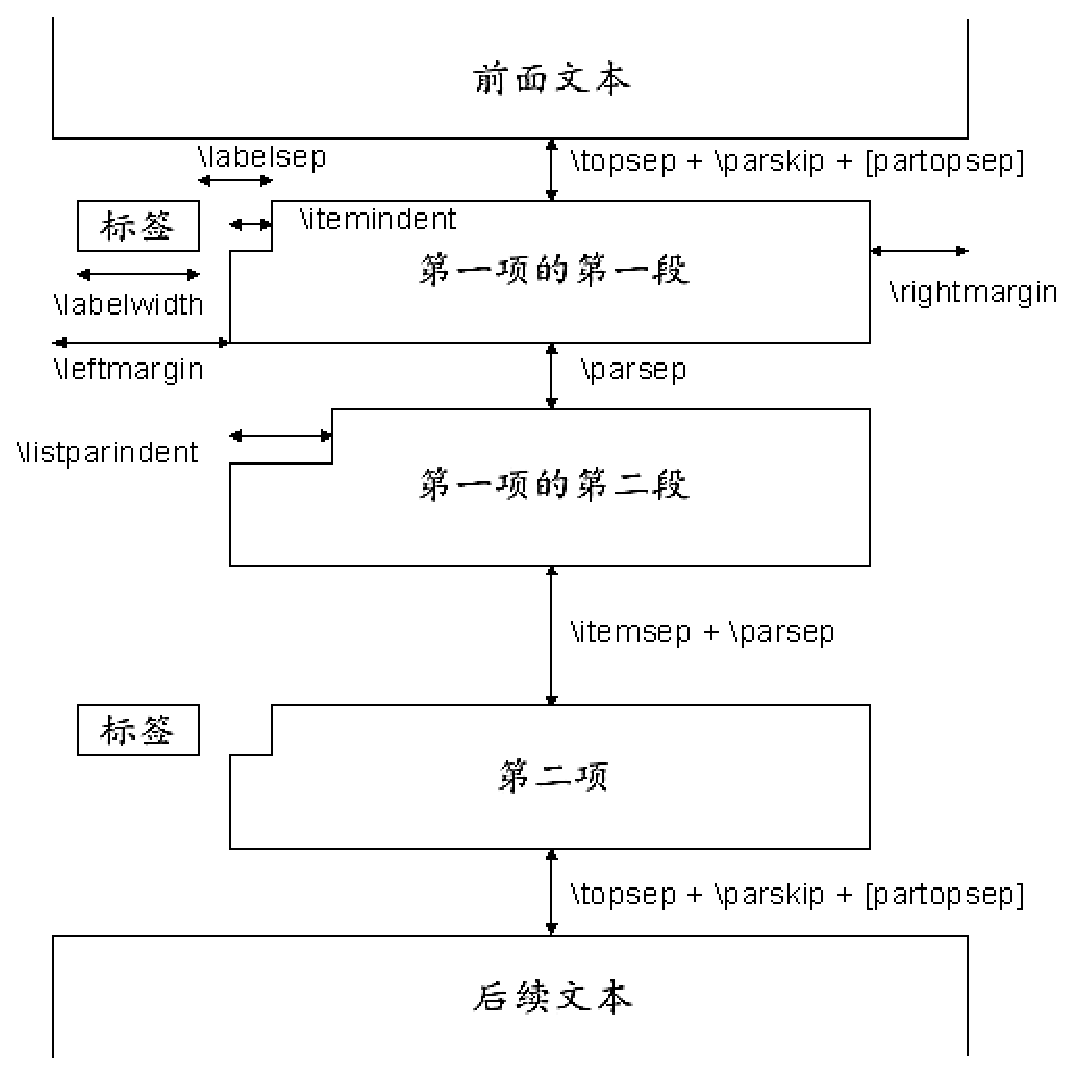
\includegraphics[width = 0.6\textwidth]{list}
\bicaption[list]{}{罗列环境参数示意图}{Fig.$\!$}{Schematic diagram of list environments}\vspace{-1em}
\end{figure}
通过调用~enumitem~宏包可以很方便地控制罗列环境的布局,其~format.tex~文件中的~\verb|\setitemize|~和~\verb|\setenumerate|~命令分别用来设置~\verb|itemize|~和~\verb|enumerate|~环境的样式参数。采用~\verb|itemize|~单层罗列环境的排版形式如下:
\begin{itemize}
\item 第一个条目文本内容
\item 第二个条目文本内容
\item 第三个条目文本内容
\end{itemize}
其代码如下
\begin{verbatim}
\begin{itemize}
  \item 第一个条目文本内容
  \item 第二个条目文本内容
  ...
  \item 第三个条目文本内容
\end{itemize}
\end{verbatim}
采用~\verb|enumerate|~单层罗列环境的排版形式如下:
\begin{enumerate}
\item 第一个条目文本内容
\item 第二个条目文本内容
\item 第三个条目文本内容
\end{enumerate}
其代码如下
\begin{verbatim}
\begin{enumerate}
  \item 第一个条目文本内容
  \item 第二个条目文本内容
  ...
  \item 第三个条目文本内容
\end{enumerate}
\end{verbatim}

\BiSection{算法}{Algorithm}

这是一个算法的例子,来自~worldguy@lilacbbs。建议将算法放在~minipage~环境中,避免算法出现在页面版心之外。

\begin{algorithm}
\KwIn{training samples, {$(d_i, d_j)_q$; $\mathbf{q}_i, \mathbf{q}_j \in C$,
$q\in \mathbf{Q}$} }
\KwOut{parameter setting $\lambda^T$}%

\For{$t$=1 to $T$}
{   
    $\lambda^{t+1}_n = \lambda^t_n + \eta (f_n(q, c, d_i) - f_n(q, c, d_j))$
 }
\end{algorithm}

%\KwIn{training samples, {$(d_i, d_j)_q$; $\mathbf{q}_i, \mathbf{q}_j \in C$,
%$q\in \mathbf{Q}$} }
%\KwOut{parameter setting $\lambda^T$}%
%
%\For{$t$=1 to $T$}
%{   
%    $\lambda^{t+1}_n = \lambda^t_n + \eta (f_n(q, c, d_i) - f_n(q, c, d_j))$
% }
%\end{algorithm}

算法环境中右侧空白比较多,若想把右侧的空白框减小,可以采用~minipage~环境实现。把~algorithm~环境放到~minipage~环境里面,并且加上选项[H]禁止算法浮动,下面给出一个例子。需要说明的是,一般不需要进行这种处理。算法标题可有可无,若有中英文标题,请使用~\verb|\AlgoBiCaption{中文标题}{英文标题}|。下面给出两个有标题的例子。需要说明的是,算法的标题是自动换行,没有必要手动换行。

\begin{minipage}{0.8\textwidth}\centering
\begin{algorithm}[H]
 \AlgoBiCaption{这是一个简短的算法中文图题}{This is the English caption of the algorithm}
  \KwIn{training samples, {$(d_i, d_j)_q$; $\mathbf{q}_i, \mathbf{q}_j
      \in C$, $q\in \mathbf{Q}$} }
 \KwOut{parameter setting
    $\lambda^T$}
 \For{$t$=1 to $T$} { $\lambda^{t+1}_n = \lambda^t_n +
    \eta (f_n(q, c, d_i) - f_n(q, c, d_j))$ }
\end{algorithm}
\end{minipage}


\begin{minipage}{0.9\textwidth}\centering
\begin{algorithm}[H]
 \AlgoBiCaption{这是一个算法的比较长的中文图题,需要换行,这里采用自动换行,如果手动换行会造成算法目录中同样出现断行}{This is a long English caption of the algorithm, a new line  required, and this a new line}
  \KwIn{training samples, {$(d_i, d_j)_q$; $\mathbf{q}_i, \mathbf{q}_j
      \in C$, $q\in \mathbf{Q}$} }
 \KwOut{parameter setting
    $\lambda^T$}
 \For{$t$=1 to $T$} { $\lambda^{t+1}_n = \lambda^t_n +
    \eta (f_n(q, c, d_i) - f_n(q, c, d_j))$ }
\end{algorithm}
\end{minipage}

\BiSection{定理定义}{Theorem and definition}

若需要书写定理定义等内容,而且带有顺序编号,需要采用如下环境。除了~\verb|proof|~环境之外,其余~9~个环境都可以有一个可选参数作为附加标题。

\begin{center}\vspace{0.5em}\noindent\wuhao\begin{tabularx}{0.7\textwidth}{lX|lX}
定理 & \verb|theorem|~环境 & 定义 & \verb|definition|~环境 \\
例 & \verb|example|~环境 & 算法 & \verb|algo|~环境 \\
公理 & \verb|axiom|~环境 & 命题 & \verb|proposition|~环境 \\
引理 & \verb|lemma|~环境 & 推论 & \verb|corollary|~环境 \\
注解 & \verb|remark|~环境 & 证明 & \verb|proof|~环境 \\
\end{tabularx}\end{center}
%% !Mode:: "TeX:UTF-8" 

\BiAppendixChapter{结\quad 论}{Conclusions}

学位论文的结论作为论文正文的最后一章单独排写,但不加章标题序号。

结论应是作者在学位论文研究过程中所取得的创新性成果的概要总结,不能与摘要混为一谈。博士学位论文结论应包括论文的主要结果、创新点、展望三部分,在结论中应概括论文的核心观点,明确、客观地指出本研究内容的创新性成果(含新见解、新观点、方法创新、技术创新、理论创新),并指出今后进一步在本研究方向进行研究工作的展望与设想。对所取得的创新性成果应注意从定性和定量两方面给出科学、准确的评价,分(1)、(2)、(3)…条列出,宜用“提出了”、“建立了”等词叙述。   % 结论

%\BiChapter{图片的插入方法}{Methods of inserting figures}

\BiSection{单张图片的插入方法}{The method of inserting one single figure}

\BiSubsection{条标题}{The caption of subsection}

单张图片独自占一行的插入形式如图~\ref{golfer1}~所示。
\begin{figure}[htbp]
\centering
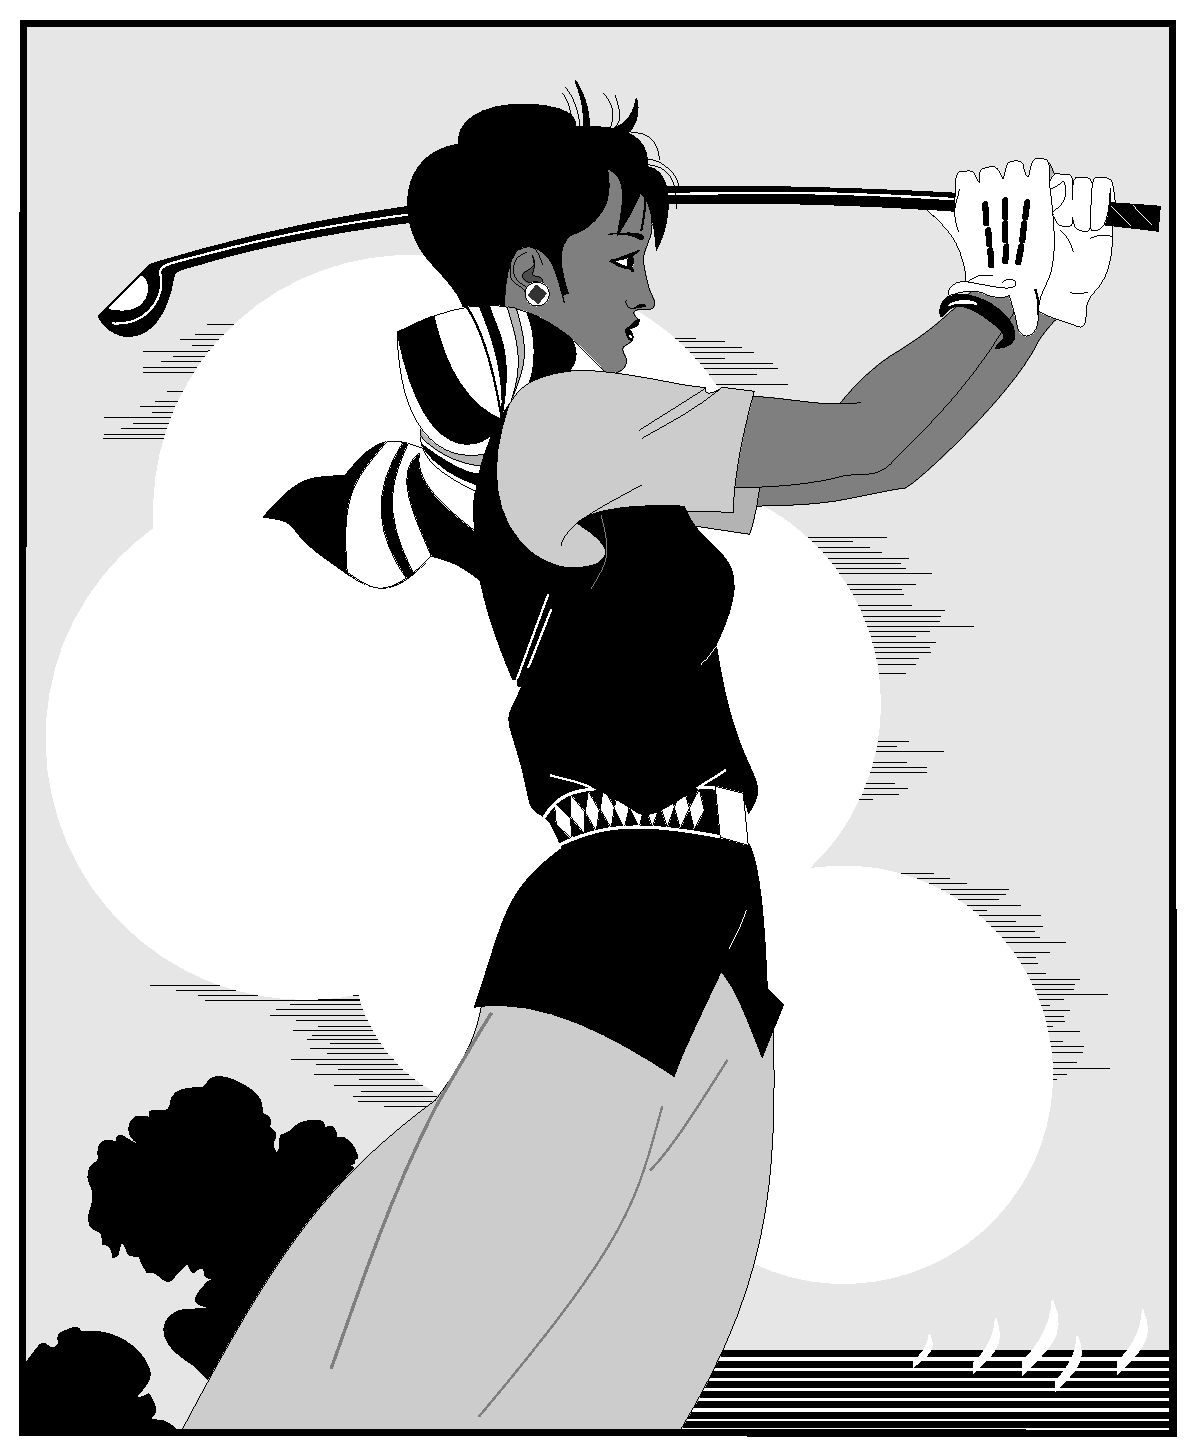
\includegraphics[width = 0.4\textwidth]{golfer}
\bicaption[golfer1]{}{打高尔夫球的人}{Fig.$\!$}{The person playing golf}\vspace{-1em}
\end{figure}

其插入图片的代码及其说明如下。
\begin{verbatim}
\begin{figure}[htbp]
\centering
\includegraphics[width=0.4\textwidth]{文件名(.eps)}
\bicaption[标签名(英文)]{}{中文标题}{Fig.$\!$}
          {English caption (首字母大写)}\vspace{-1em}
\end{figure}
\end{verbatim}
%\BiChapter{表格的绘制方法}{Methods of drawing tables}

\BiSection{普通表格的绘制方法}{Methods of drawing normal tables}


表格应具有三线表格式,因此需要调用~booktabs~宏包,其标准格式如表~\ref{table1}~所示。
\begin{table}[htbp]
\bicaption[table1]{}{符合研究生院绘图规范的表格}{Table$\!$}{Table in agreement of the standard from graduate school}
\vspace{0.5em}\centering\wuhao
\begin{tabular}{ccccc}
\toprule[1.5pt]
$D$(in) & $P_u$(lbs) & $u_u$(in) & $\beta$ & $G_f$(psi.in)\\
\midrule[1pt]
 5 & 269.8 & 0.000674 & 1.79 & 0.04089\\
10 & 421.0 & 0.001035 & 3.59 & 0.04089\\
20 & 640.2 & 0.001565 & 7.18 & 0.04089\\
\bottomrule[1.5pt]
\end{tabular}
\end{table}

其绘制表格的代码及其说明如下。
\begin{verbatim}
\begin{table}[htbp]
\bicaption[标签名]{}{中文标题}{Table$\!$}{English caption}
\vspace{0.5em}\centering\wuhao
\begin{tabular}{cc...c}
\toprule[1.5pt]
表头第1个格   & 表头第2个格   & ... & 表头第n个格  \\
\midrule[1pt]
表中数据(1,1) & 表中数据(1,2) & ... & 表中数据(1,n)\\
表中数据(2,1) & 表中数据(2,2) & ... & 表中数据(2,n)\\
...................................................\\
表中数据(m,1) & 表中数据(m,2) & ... & 表中数据(m,n)\\
\bottomrule[1.5pt]
\end{tabular}
\end{table}
\end{verbatim}
%\BiChapter{数学公式的输入方法}{Input methods of equations}

\BiSection{行内公式}{Inline mode equations}

出现在正文一行之内的公式称为行内公式,例如~$f(x)=\int_{a}^{b}\frac{\sin{x}}{x}\mathrm{d}x$。对于非矩阵和非多行形式的行内公式,一般不会使得行距发生变化。

\BiSection{行间公式}{Displaymath mode equations}

位于两行之间的公式称为行间公式,每个公式都是一个单独的段落,下边的例子是一个无编号的行间单行公式

\[
\int_a^b{f\left(x\right)\mathrm{d}x}=\lim_{\left\|\Delta{x_i}\right\|\to 0}\sum_i{f\left(\xi_i\right)\Delta{x_i}}
\]

下边的例子是一个无编号的行间多行公式(\ref{lizi})
\begin{eqnarray*}\label{lizi}
\sin 2x&=&2\sin x\cos x\\
\cos 2x&=&2\cos x^2-1=1-2\sin x^2=\cos x^2-\sin x^2
\end{eqnarray*}
%参考文献\cite{OOSTRUM01}和参考文献\citeup{wwwlixing}


%参考文献
\defaultfont
\bibliographystyle{GBT7714-2005NLang-HIT}
\addcontentsline{toc}{chapter}{参考文献}      % 参考文献加入到中文目录
\addcontentsline{toe}{chapter}{\bfseries  REFERENCES} % 参考文献加入到英文目录
\addtolength{\bibsep}{-0.8em}
%\nocite{*}  %若将此命令屏蔽掉,则未引用的文献不会出现在文后的参考文献列表中。
%\bibliography{reference.bib}
\bibliography{MyCollection.bib}
%\bibliography{nongzhong.
%% -*-coding: utf-8 -*-

\defaultfont
\appendix

%%%%%%%%%%%%%%%%%%%%%%%%%%%%%%%%%%%%%%%%%%%%%%%%%%%%%%%%%
\BiAppChapter{带章节的附录}{Full Appendix}%
完整的附录内容,包含章节,公式,图表等

%%%%%%%%%%%%%%%%%%%%%%%%%%%%%%%%%%%%%%%%%%%%%%%%%%%%%%%%%
\BiSection{附录节的内容}{Section in Appendix}
这是附录的节的内容

附录中图的示例:
\begin{figure}[htbp]
\centering
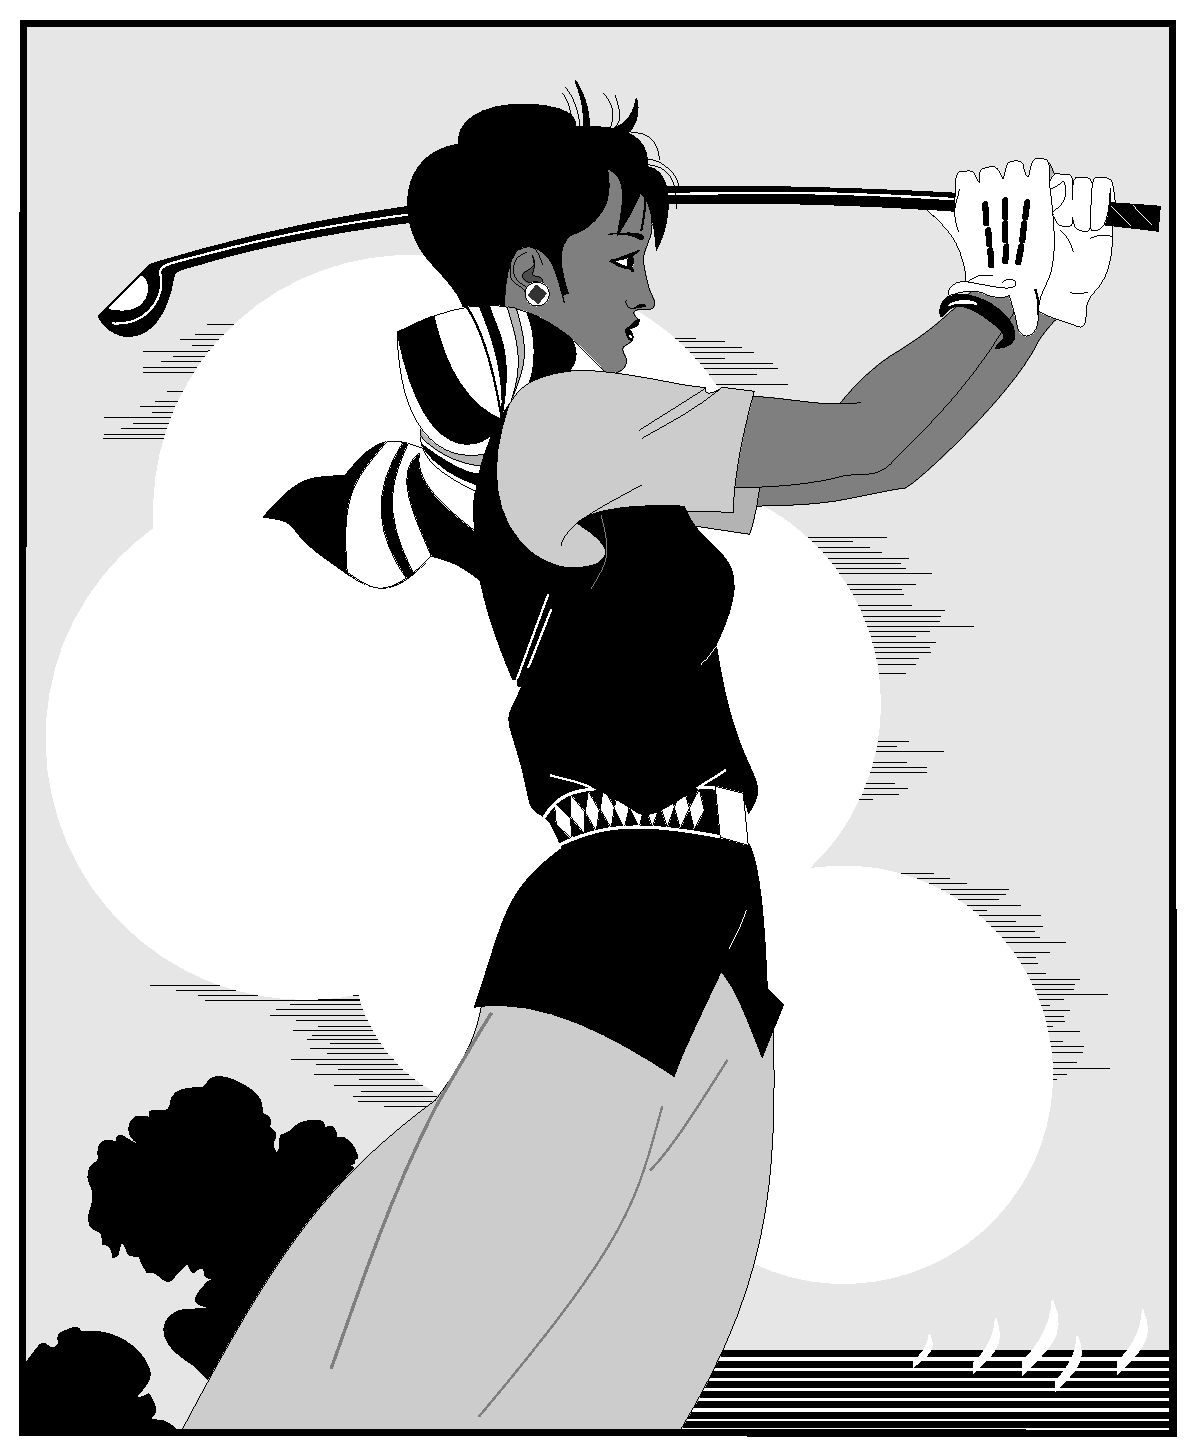
\includegraphics[width = 0.4\textwidth]{golfer}
\bicaption[golfer5]{}{打高尔夫球的人}{Fig.$\!$}{The person playing golf}\vspace{-1em}
\end{figure}

附录中公式的示例:
\begin{align}
a & = b \times c \\
E & = m c^2
\end{align}






%\BiAppChapter{附录三}{appendix 3}    % 附录
%% !Mode:: "TeX:UTF-8" 

\BiAppendixChapter{攻读\cxuewei 学位期间发表的论文及其他成果} {Papers
published in the period of PH.D. education}
\noindent\textbf{(一)发表的学术论文}
\begin{publist}
\item	\underline{XXX},XXX. Static Oxidation Model of Al-Mg/C Dissipation Thermal Protection Materials[J]. Rare Metal Materials and Engineering, 2010, 39(Suppl. 1): 520-524.(SCI~收录,IDS号为~669JS,IF=0.16)
\item XXX,\underline{XXX}. 精密超声振动切削单晶铜的计算机仿真研究[J]. 系统仿真学报,2007,19(4):738-741,753.(EI~收录号:20071310514841)
\item XXX,XXX. 局部多孔质气体静压轴向轴承静态特性的数值求解[J]. 摩擦学学报,2007(1):68-72.(EI~收录号:20071510544816)
\item XXX,XXX. 硬脆光学晶体材料超精密切削理论研究综述[J]. 机械工程学报,2003,39(8):15-22.(EI~收录号:2004088028875)
\item XXX,XXX. 基于遗传算法的超精密切削加工表面粗糙度预测模型的参数辨识以及切削参数优化[J]. 机械工程学报,2005,41(11):158-162.(EI~收录号:2006039650087)
\item XXX,XXX. Discrete Sliding Mode Cintrok with Fuzzy Adaptive Reaching Law on 6-PEES Parallel Robot[C]. Intelligent System Design and Applications, Jinan, 2006: 649-652.(EI~收录号:20073210746529)
\end{publist}

\noindent\textbf{(二)申请及已获得的专利(无专利时此项不必列出)}
\begin{publist}
\item XXX,XXX. 一种温热外敷药制备方案:中国,88105607.3[P]. 1989-07-26.
\end{publist}

\noindent\textbf{(三)参与的科研项目及获奖情况}
\begin{publist}
\item	XXX,XXX. XX~气体静压轴承技术研究, XX~省自然科学基金项目.课题编号:XXXX.
\item XXX,XXX. XX~静载下预应力混凝土房屋结构设计统一理论. 黑江省科学技术二等奖, 2007.
\end{publist}
%\vfill
%\hangafter=1\hangindent=2em\noindent

%\setlength{\parindent}{2em}
    % 所发文章
%% !Mode:: "TeX:UTF-8" 

\BiAppendixChapter{学位论文原创性声明和使用权限}{Statement of copyright and Letter of authorization}
\vspace{\baselineskip}
\begin{center}\hei\xiaosan{学位论文原创性声明}\end{center}
\vspace{1em}

本人郑重声明:此处所提交的学位论文,是本人在导师指导下,在XXX大学攻读学位期间独立进行研究工作所取得的成果,且学位论文中除已标注引用文献的部分外不包含他人完成或已发表的研究成果。对本学位论文的研究工作做出重要贡献的个人和集体,均已在文中以明确方式注明。

\vspace{\baselineskip}
\hspace{6em}作者签名:\hfill 日期:\hspace{2.5em}年\hspace{1.5em}月\hspace{1.5em}日

\vspace{2\baselineskip}
\begin{center}\hei\xiaosan{学位论文使用权限}\end{center}
\vspace{1em}

学位论文是研究生在XXXXX大学攻读学位期间完成的成果,知识产权归属XXXXX大学。学位论文的使用权限如下:

(1)学校可以采用影印、缩印或其他复制手段保存研究生上交的学位论文,并向国家图书馆报送学位论文;(2)学校可以将学位论文部分或全部内容编入有关数据库进行检索和提供相应阅览服务;(3)研究生毕业后发表与此学位论文研究成果相关的学术论文和其他成果时,应征得导师同意,且第一署名单位为XXXX大学。

保密论文在保密期内遵守有关保密规定,解密后适用于此使用权限规定。

本人知悉学位论文的使用权限,并将遵守有关规定。


\vspace{2\baselineskip}
\hspace{6em}作者签名:\hfill 日期:\hspace{2.5em}年\hspace{1.5em}月\hspace{1.5em}日

\vspace{2\baselineskip}
\hspace{6em}导师签名:\hfill 日期:\hspace{2.5em}年\hspace{1.5em}月\hspace{1.5em}日   % 承诺
% !Mode:: "TeX:UTF-8" 



% 致谢

\ifxueweidoctor
% !Mode:: "TeX:UTF-8" 

\defaultfont

\BiAppendixChapter{个人简历}{Resume}

XXXX~年~XX~月~XX~日出生于~XXXX。

XXXX~年~XX~月考入~XX~大学~XX~院(系)XX~专业,XXXX~年~XX~月本科毕业并获得~XX~学学士学位。

XXXX~年~XX~月------XXXX~年~XX~月在~XX~大学~XX~院(系)XX~学科学习并获得~XX~学硕士学位。

XXXX~年~XX~月------XXXX~年~XX~月在~XX~大学~XX~院(系)XX~学科学习并获得~XX~学博士学位。

获奖情况:如获三好学生、优秀团干部、X~奖学金等(不含科研学术获奖)。

工作经历:

\vspace{3em}\noindent
\textbf{( 除全日制硕士生以外,其余学生均应增列此项。个人简历一般应包含教育经历和工作经历。)}          % 博士学位论文有个人简介
\fi

\clearpage

\end{document} 
